\documentclass[9pt,aspectratio = 169]{beamer}

\usepackage[brazil]{babel} % section and appendix headings in Portuguese
\usepackage{setspace} % line spacing
\usepackage{times} % font times new roman
\usepackage[bottom=2cm,top=3cm,left=3cm,right=2cm]{geometry} % margins ABNT
\usepackage{ragged2e} % justified text
\usepackage{graphicx} % figures
\usepackage{float} % position of contents right after text
\usepackage{subcaption}  % subcaptions for figures, tables etc
\usepackage{caption} % captions for figures, tables etc
\usepackage{hyperref} % hyperlinks for references, figures and tables
\usepackage{multirow} % multirow tables
\usepackage[alf,abnt-repeated-title-omit=yes,abnt-emphasize=bf,abnt-full-initials=no]{abntex2cite}
\citebrackets() % parenthesis brackets for citations
\setlength\parindent{0pt} % no indentation
% \renewcommand{\citeonline}{#1}

\setcounter{secnumdepth}{5} % section numbering depth
\setcounter{tocdepth}{5} % table of contents depth

\def\changemargin#1#2{\list{}{\rightmargin#2\leftmargin#1}\item[]} % paragraph margin adjustment
\let\endchangemargin=\endlist % paragraph margin adjustment

\usepackage{titlesec} % section headings format
\titleformat{name=\section,numberless}{\filcenter\normalfont\normalsize\bfseries\uppercase}{}{0em}{}
\titleformat{\section}{\normalfont\normalsize\bfseries\uppercase}{\thesection}{1em}{}
\titleformat{\subsection}{\normalfont\normalsize\uppercase}{\thesubsection}{1em}{}
\titleformat{\subsubsection}{\normalfont\normalsize\bfseries}{\thesubsubsection}{1em}{}
\titleformat{\paragraph}{\normalfont\normalsize\itshape}{\theparagraph}{1em}{}
\titleformat{\subparagraph}{\normalfont\normalsize}{\thesubparagraph}{1em}{}


\DeclareCaptionType[fileext=loc]{quadro}[Quadro][Lista de Quadros] % create float type for frames, similar to tables

\usepackage{tocbasic} % table of contents format

\DeclareTOCStyleEntry[
  entrynumberformat=\entrynumberwithprefix{\figurename},
  dynnumwidth
%   numsep=1em
]{tocline}{figure}

\DeclareTOCStyleEntry[
    entrynumberformat=\entrynumberwithprefix{\tablename},
    dynnumwidth
    %   numsep=1em
]{tocline}{table}
        
\newcommand\entrynumberwithprefix[2]{#1\enspace#2-\enspace}
\captionsetup{labelsep=endash} % caption label separator '-'

\usepackage{showframe} % just for the example
\usepackage{tocloft}

\renewcommand{\cfttoctitlefont}{\hspace*{\fill}\normalsize\bfseries\MakeUppercase}
\renewcommand{\cftaftertoctitle}{\hspace*{\fill}}
\renewcommand{\cftlottitlefont}{\hspace*{\fill}\normalsize\bfseries\MakeUppercase}
\renewcommand{\cftafterlottitle}{\hspace*{\fill}}
\renewcommand{\cftloftitlefont}{\hspace*{\fill}\normalsize\bfseries\MakeUppercase}
\renewcommand{\cftafterloftitle}{\hspace*{\fill}}


\usepackage{titletoc} % table of contents alignment
\dottedcontents{section}[2cm]{\bfseries}{2cm}{0.5pc}
\dottedcontents{subsection}[2cm]{}{2cm}{0.5pc}
\dottedcontents{subsubsection}[2cm]{\bfseries}{2cm}{0.5pc}
\dottedcontents{paragraph}[2cm]{\itshape}{2cm}{0.5pc}
\dottedcontents{subparagraph}[2cm]{}{2cm}{0.5pc}
\renewcommand{\contentsname}{\centering Contents}

%-------------------------------------------------------
% INFORMATION IN THE TITLE PAGE
%-------------------------------------------------------
 \institute{\textcolor{verde}{Programa de Pós-Graduação de Mestrado Profissional em Engenharia de Produção}}
\titlegraphic{
    \begin{picture}(0,0)
        \put(422,14){\makebox(0,0)[rt]{
\includegraphics[width=2cm]{images/logo-unifei-oficial.png}}}
    \end{picture}
}

\title[Redes neurais aplicado na previsão de índice Sharpe] % [] is optional - is placed on the bottom of the sidebar on every slide
{ % is placed on the title page
      \textbf{Redes neurais aplicado na previsão de índice Sharpe:
}
}

\subtitle[Evidência em componentes do Ibovespa]
{
    Evidência em componentes do Ibovespa\\
}

\author[Autores]
{ \normalsize \centering
        Renan Delgado Camurça Lima 
}

\institute[Unifei]
{\small 
   
    UNIVERSIDADE FEDERAL DE ITAJUBÁ \\
    CAMPUS ITABIRA \\
    MESTRADO PROFISSIONAL EM ENGENHARIA DE PRODUÇÃO \\
  
  %there must be an empty line above this line - otherwise some unwanted space is added between the university and the country (I do not know why;( )
}

\date{\centering 14 de julho de 2023}

%-------------------------------------------------------
% THE BODY OF THE PRESENTATION
%-------------------------------------------------------

\begin{document}

    %-------------------------------------------------------
    % THE TITLEPAGE
    %-------------------------------------------------------

    % % this is the name of the PDF file for the background
    \begin{frame}[plain,noframenumbering] % the plain option removes the header from the title page, noframenumbering removes the numbering of this frame only
    \titlepage % call the title page information from above
    \end{frame}


    
%-------------------------------------------------------
\begin{frame}{Visão Geral}

    \begin{itemize}
        \item \textbf{Objetivo:} Aplicar redes neurais na previsão do índice Sharpe para seleção de carteiras de investimento.
        \item \textbf{Originalidade:} Seleção de carteiras de investimento com o uso de redes neurais após otimização baseada no índice Sharpe.
        \item \textbf{Método:} Estudo empírico com dados históricos de ativos financeiros e dados econômicos aplicados em otimização de carteiras e redes neurais.
        \item \textbf{Principais descobertas:} As redes neurais, embora não superem as carteiras, demonstram desempenho superior ao Ibovespa. A estrutura de rede de \textit{LSTM}+Atenção de Bahdanau obteve o melhor desempenho.
        \item \textbf{Implicação teórica e prática:} Contribui para o avanço do conhecimento na área de finanças e destaca o potencial das redes neurais na seleção de carteiras de investimento. Além disso, as peças de códigos geradas permitem a aplicação em outros estudos.
        \item \textbf{Palavras-chave:} Redes neurais, Índice Sharpe, Otimização de Carteiras.
    \end{itemize}

\end{frame}
\note{

    A aplicação de modelos de redes neurais com intuito de selecionar ativos para carteiras de investimentos com o uso do índice Sharpe é uma área que atrai a atenção de pesquisadores. Este estudo visa aplicar redes neurais na previsão do índice Sharpe para seleção de carteiras de investimento. Através de uma revisão bibliográfica, são identificados os métodos utilizados na construção de carteiras, assim como as técnicas de otimização e as estruturas de redes neurais empregadas nesse contexto. A construção dos modelos de previsão requer a coleta e o tratamento de dados históricos de ativos financeiros e dados econômicos. O processo de seleção de carteiras é dividido em duas etapas: a otimização baseada no índice Sharpe e a seleção da carteira utilizando redes neurais para previsão da carteira com melhor desempenho no período seguinte. A avaliação do desempenho é realizada em comparação com o índice Bovespa. Os resultados mostram que o modelo sem restrições apresenta melhor desempenho em tempo de otimização e índice Sharpe. As redes neurais, embora não superem as carteiras, demonstram desempenho superior ao Ibovespa. A rede neural LSTM+Atenção de Bahdanau obteve o melhor desempenho. Essas descobertas contribuem para o avanço do conhecimento na área de finanças e destacam o potencial das redes neurais na seleção de carteiras de investimento.

}
%-------------------------------------------------------


    \begin{frame}{Agenda}{}
        \tableofcontents
    \end{frame}

    %-------------------------------------------------------
\section{Introdução}
%-------------------------------------------------------


%-------------------------------------------------------
    \begin{frame}{Teoria Moderna de Portfólio e Índice Sharpe}
        
        \LARGE \textbf{Teoria moderna de portfólio \cite{markowitz1952portfolio}.}

        \Large
        % side by side text and figure
        \begin{columns}
            \begin{column}{0.5\textwidth}
                \begin{itemize}
                    \item Gestão de investimentos \cite{sethi2021nobel}.
                    \item Risco e retorno \cite{sharpe1964capital}.
                    \item Diversificação e preferência \cite{lintner1965valuation}.
                    \item Prêmio por unidade de risco \cite{sharpe1994sharpe}.
                \end{itemize}

            \end{column}
            \begin{column}{0.5\textwidth}
                \begin{figure}
                    \centering
                    \caption{Fronteira eficiente e Linha de Mercado}
                    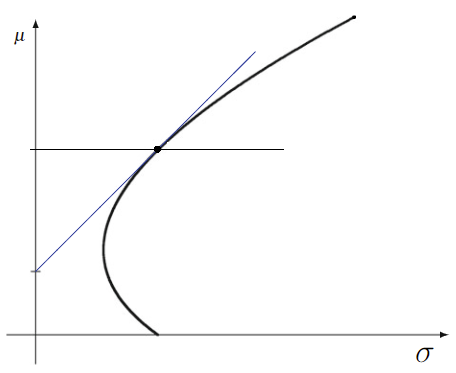
\includegraphics[width=0.6\textwidth]{images/fronteira_eficiente.png}
                    \par \footnotesize Fonte: adaptado \citeauthor{mansini2015linear}.
                \end{figure}
            \end{column}
        \end{columns}
        

    \end{frame}
    \note{    

        \ipar O mercado financeiro gerencia trilhões de dólares com uso da teoria moderna de portfólios elaborada pelo laureado do prêmio Nobel de economia Harry Markowitz \cite{sethi2021nobel}. As discussões sobre a teoria foram aprofundadas pelo também laureado William Sharpe, que aborda a estratégia de maximização de uma carteira de investimentos, considerando tanto o risco quanto o retorno. 
                
        \ipar A intuição do investidor seria que a máxima diversificação para um retorno esperado da carteira geraria um portfólio de mínima variância, isto é, com menor risco. Contudo, esta hipótese é rejeitada segundo a teoria de \citeonline{markowitz1952portfolio}, pois existe uma combinação ideal de ativos que compõem uma carteira de forma eficiente maximizando o retorno com o menor nível de risco. Portanto, a cada retorno esperado há uma combinação eficiente dos ativos que gera uma carteira de mínima variância, assim formando uma fronteira eficiente de combinações de ativos.

        \ipar A escolha da carteira eficiente é feita com base na relação entre risco e retorno. Segundo \citeonline{sharpe1964capital}, os investidores exigem um prêmio de retorno para assumir riscos adicionais. Desta maneira, a preferência dá-se pela aceitação ao risco, em que para opções de investimentos com o mesmo retorno esperado, o investidor escolherá a opção com menor risco \cite{lintner1965valuation}.

        \ipar Este prêmio por unidade de risco é conhecido como o índice Sharpe \cite{sharpe1994sharpe}. O termo foi apresentado por \citeonline{treynor1973use} em reconhecimento as contribuições feitas na avaliação de desempenho de fundos feita por \citeonline{sharpe1966mutual}, e atualmente é uma das medidas mais utilizadas para avaliação de desempenho de carteiras de investimento.

        \ipar Considerando que existe a opção para o investidor realizar empréstimo ou tomar emprestado a uma taxa livre de risco, é possível construir uma carteira eficiente que combina o empréstimo com todos os investimentos disponíveis no mercado. Esta combinação forma uma linha reta que tangencia a fronteira eficiente de ativos. Esta linha é denominada linha do mercado de capitais, e a carteira eficiente que tangencia a linha é chamada de carteira de mercado, que apresenta o maior prêmio por unidade risco \cite{sharpe1964capital}.

    }
%-------------------------------------------------------



%-------------------------------------------------------
    \begin{frame}{Séries Temporais e Redes Neurais}

        \LARGE \textbf{Otimização de Carteiras de Investimentos}

        \vspace{1cm}


            % side by side text and figure
            \begin{columns}
                \begin{column}{0.5\textwidth}
                    
                    \LARGE \textbf{Modelos Tradicionais \cite{zhou2023twostage}}

                    \Large
                    \begin{itemize}
                        \item Métodos estatísticos.
                        \item Séries temporais lineares.
                        \item \textit{ARIMA}.
                    \end{itemize}
                    \vspace{11pt}

                \end{column}
                \begin{column}{0.5\textwidth}
                    \LARGE \textbf{Novos Estudos}

                    \Large
                    \begin{itemize}
                        \item Aprendizado de máquina.
                        \item Séries temporais não lineares.
                        \item Redes neurais.
                        \item \textit{LSTM}.
                    \end{itemize}
                            
                \end{column}
            \end{columns}
            


    \end{frame}
    \note{
        
        Modelos Tradicionais -> Não linearidade -> Redes Neurais
        
        \ipar Uma estratégia de construção de carteira de investimentos é a otimização do índice Sharpe, que consiste em maximizar o índice Sharpe para uma carteira de ativos para obter a carteira de mercado \cite{maree2022balancing}. Para a otimização da carteira é necessário estimar o retorno e o risco da carteira. A estimativa do retorno esperado é feita com base em dados históricos, e o risco é estimado com base na matriz de correlação dos ativos e a volatilidade de cada ativo.

        \ipar Modelos de otimização também combinam previsão das séries temporais para estimar o retorno esperado da carteira. Modelos tradicionais de previsão de séries temporais, aplicam métodos estatísticos que consideram as séries como modelos lineares \cite{zhou2023twostage}. Dentre estes há os modelos de médias móveis auto-regressivas integradas (\acrshort{ARIMA}, do inglês \textit{Autoregressive Integrated Moving Average}), e heterocedasticidade condicional autoregressiva generalizada (\acrshort{GARCH}, do inglês \textit{Generalized Autoregressive Conditional Heterocedasticity}). 
        
        \ipar Entretanto, séries temporais de ativos financeiros como ações, apresentam uma dinâmi-ca de processo não linear. Há diversas abordagens para capturar dados não lineares, dentre estes há as redes neurais artificiais, modelos de redes neurais profundas, ou a rede neural recorrente que se provaram como ferramentas válidas para aplicações para dados de séries temporais multivariada \cite{cao2020delafo}. Além disso, os modelos podem ser combinados com métodos de otimização para a seleção de carteiras de investimentos \cite{du2022mean}.

        \ipar A aplicação de modelos de redes neurais com intuito de selecionar ativos para carteiras de investimentos é uma área que tem atraído a atenção de pesquisadores. O índice Sharpe tem sido utilizado em estudos como a função objetivo para a otimização de carteiras de investimentos com modelos de redes neurais \cite{tran2023optimizing}. Além disso, estuda-se a aplicação de redes neurais para predição do maior índice Sharpe no futuro \cite{vukovic2020neural}.

        \ipar Em geral, as redes neurais recorrentes (\acrshort{RNN}, do inglês \textit{Recurrent Neural Network}) têm se mostrado eficientes para previsão de séries temporais de ações \cite{wang2020portfolio}, em especial memória de longo prazo com curto prazo (\acrshort{LSTM}, do inglês \textit{Long Short-Term Memory}). Estes modelos de redes neurais utilizam uma camada de memória que permite a rede aprender dependências de longo prazo, e são capazes de capturar padrões de séries temporais não lineares para realizar previsões \cite{hochreiter1997long}.

        \ipar Há a possibilidade de combinar estruturas de redes neurais entre si para obter melhores resultados. O mecanismo de atenção tem sido efetivamente aplicado na área de processamento de linguagem natural, tem sido utilizado para melhorar o desempenho de modelos de redes neurais para previsão de séries temporais. Como exemplo, \citeonline{sun2022deep} desenvolveu um modelo para as séries temporais que combina uma rede neural convolucional com um transformador (rede neural baseada no mecanismo de atenção) para otimização de uma carteira de investimentos com objetivo de maximização do índice Sharpe.


    }
%-------------------------------------------------------





%-------------------------------------------------------
    \begin{frame}{Otimização e Redes Neurais}

        \LARGE \textbf{Otimização de Carteiras de Investimentos com Índice Sharpe}

        Combinação de redes neurais e otimização:

        \begin{itemize}
            \item \citeauthor{vukovic2020neural}(\citeyear{vukovic2020neural}): Perceptron multicamada para predição de ETF com melhor Índice Sharpe.
            \item \citeauthor{sun2022deep}(\citeyear{sun2022deep}): Redes Convolucionais com Atenção para otimização de carteiras por reforço com índice Sharpe.
            \item \citeauthor{cao2020delafo}(\citeyear{cao2020delafo}): Redes Recorrentes com Atenção para otimização de carteiras por reforço com índice Sharpe.
        \end{itemize}
                    

    \end{frame}
    \note{
        
        Combinação, complexidade e restrições reais

        \ipar Há a possibilidade de combinar estruturas de redes neurais entre si para obter melhores resultados. O mecanismo de atenção tem sido efetivamente aplicado na área de processamento de linguagem natural, tem sido utilizado para melhorar o desempenho de modelos de redes neurais para previsão de séries temporais. Como exemplo, \citeonline{sun2022deep} desenvolveu um modelo para as séries temporais que combina uma rede neural convolucional com um transformador (rede neural baseada no mecanismo de atenção) para otimização de uma carteira de investimentos com objetivo de maximização do índice Sharpe.

        \ipar Em modelos de otimização há restrições e parâmetros que podem ser adicionados para tornar o problema próximo ao real. \citeonline{mulvey2020optimizing} propõe um modelo de otimização de carteira de investimentos com redes neurais que considera a taxa de transação. 
        
        \ipar A aplicação de restrições como a taxa de transação, limitação de capital, e restrições como a de cardinalidade, que limita o número de ativos na carteira tornam o problema próximo da realidade, contudo aumentam a complexidade de resolução \cite{aithal2023real}. Uma abordagem para resolução de problemas complexos é a utilização de métodos heurísticos, que são métodos de busca que não garantem a solução ótima, mas são capazes de encontrar soluções próximas da ótima em um tempo computacionalmente viável \cite{milhomem2020analysis}.

        \ipar Os estudos sobre otimização de carteiras de investimentos pelo índice Sharpe têm apresentado somente uma restrição real, o efeito do custo de transação. Em maioria negligenciam questões como lote padrão, a aversão ao risco e outras restrições afetam a decisão sobre a alocação de ativos. Estes parâmetros seguem as regulações e práticas exercidas no mercado em que se inserem.

        \ipar O índice Bovespa (\acrshort{IBOVESPA}) é o principal indicador de desempenho das ações do mercado de capitais brasileiro e referência para investidores, reunindo as empresas mais importantes do mercado nacional. A composição do ativo é construída com base nos seguintes critérios: quanto ao volume financeiro no mercado a vista, quanto índice de negociabilidade e presença no pregão, e quanto ao valor do ativo \cite{B32023}. 

    }
%-------------------------------------------------------


%-------------------------------------------------------
    \begin{frame}{Objetivos}

        \Large 

        Avaliação da aplicação de redes neurais para previsão de índice Sharpe para seleção de carteiras de investimentos
    
        \begin{itemize}
            \item Revisão sistemática.
            \item Ferramenta para coleta de dados.
            \item Modelo de alocação incluindo parâmetros reais.
            \item Estruturas de redes neurais.
            \item Analisar o desempenho da seleção. 
        \end{itemize}


    \end{frame}
    \note{
            
        \ipar Este processo é complexo e demanda tempo e conhecimento do investidor. A aplicação de modelos de redes neurais para previsão de índice Sharpe pode auxiliar o investidor a tomar decisões de alocação de ativos, e a prever o desempenho de sua carteira de investimentos. 

        \ipar Logo, a contribuição deste trabalho é o desenvolvimento de uma ferramenta de seleção de carteiras de investimentos com a construção de um fluxo de processamento que permita o investidor obter uma carteira de investimento para a sua realidade, com base em um modelo de risco e retorno, e com a aplicação de redes neurais para previsão de índice Sharpe. 

        \ipar O objetivo principal deste trabalho é desenvolver e analisar uma estrutura que aplica redes neurais para previsão de índice Sharpe para seleção de carteiras de investimento.

        \ipar Para o desenvolvimento e análise de modelos seleção de carteiras de investimento, é necessário avaliar as referências historicamente mais relevantes e identificar estudos recentes sobre o tema. A partir da revisão bibliográfica, é possível identificar os métodos utilizados para construção de carteiras. Assim, busca-se identificar as tecnologias referentes a avaliação de risco e retorno para construção de carteiras de investimentos, identificar as técnicas de otimização para previsão de índice Sharpe e as estruturas de redes neurais para seleção de carteiras.

        \ipar A construção dos modelos são dependentes de dados históricos de ativos financeiros e dados de mercado. Portanto, é necessário a coleta de dados históricos de ativos financeiros e dados econômicos de forma estruturada e com qualidade de dados. Além disso, há a preocupação de tratamento e preparação dos dados, devido a não padronização das diferentes fontes.

        \ipar A partir da construção dos modelos, é necessário avaliar o desempenho da seleção de carteiras de investimentos. Para isso, o processo tem duas etapas principais: a otimização de carteiras de investimentos pela maximização do índice Sharpe, e a seleção da carteira de investimentos com base em redes neurais pela previsão de índice Sharpe. 

        \ipar A primeira etapa incorpora a construção de carteiras de investimentos com base em modelos de risco e retorno. Busca-se avaliar a  aplicação de parâmetros reais, como capital investido, custo de transação, rebalanceamento, lotes padrão, aversão a risco e cardinialidade. Para resolução, avalia-se métodos de otimização de programação não linear. Contudo, dado a complexidade do problema, faz-se necessário a avaliação de método heurístico para resolução.

        \ipar A segunda etapa incorpora a construção de redes neurais para previsão de índice Sharpe. Para isso, busca-se avaliar diferentes estruturas de redes neurais afim de identificar a que melhor se adequa ao problema. Estas redes passam por etapas de treinamento e validação com objetivo de avaliar o desempenho da rede neural.

        \ipar Por fim, avalia-se o desempenho da seleção de carteiras de investimentos aplicados a este fluxo de processamento de duas etapas. Portanto, seguindo as etapas descritas, de revisão, coleta, modelagem e análise tem-se a avaliação da aplicação de redes neurais para previsão de índice Sharpe para seleção de carteiras de investimentos.



        \begin{enumerate}
            \item Realizar uma revisão sistemática da literatura sobre seleção de carteiras de investimentos, com base em modelos de risco e retorno, e com base em redes neurais.
            \item Construir ferramenta para coleta de dados históricos de ativos financeiros e dados econô-micos de forma estruturada e com qualidade de dados.
            \item Desenvolver um modelo de alocação de ativos baseado no cálculo do índice Sharpe e com base em modelos de risco e retorno incluindo parâmetros reais.
            \item Elaborar estruturas de redes neurais para previsão de índice Sharpe e seleção da melhor carteira de investimentos.
            \item Analisar o desempenho da seleção de carteiras de investimentos aplicados a este fluxo de processamento de duas etapas. 
        \end{enumerate}


    }
%-------------------------------------------------------



    %-------------------------------------------------------
\section{Fundamentação Teórica}
%-------------------------------------------------------




%-------------------------------------------------------
    \begin{frame}{Análise de Revisão Sistemática}


        \Large
        % side by side text and figure
        \begin{columns}
            \begin{column}{0.65\textwidth}

                \begin{quadro}[htbp]
                    \centering
                    \caption{Referências mais citadas pelos documentos selecionados}
                    \label{quadro:citados}
                    \resizebox{.9\columnwidth}{!}{%
                    \begin{tabular}{p{0.45\linewidth}cp{\linewidth}}
                        \hline 
                        Referência citada & Citações & Visão Geral \\ \hline \hline
                        \citeauthor{markowitz1952portfolio} \citeyear{markowitz1952portfolio} & 31 & Teoria Moderna de Portfólio. \\ \hline
                        \citeauthor{almahdi2017adaptive}\citeyear{almahdi2017adaptive} & 8 & Alocação de carteira utilizando aprendizagem por reforço recorrente com máximo \textit{drawdown}. \\ \hline
                        \citeauthor{hochreiter1997long}\citeyear{hochreiter1997long} & 8 & Redes neurais recorrentes LSTM. \\ \hline
                        \citeauthor{kolm2014years}\citeyear{kolm2014years} & 8 & Revisão de 60 anos da teoria de otimização de portfólio. \\ \hline
                        \citeauthor{demiguel2009optimal}\citeyear{demiguel2009optimal} & 7 & Comparação de portfólio ótimo com modelo uniforme $1/N$. \\ \hline
                        \citeauthor{fischer2018deep}\citeyear{fischer2018deep} & 7 & Previsão de movimento de mercado com LSTM aplicado a grande dimensionalidade. \\ \hline
                        \citeauthor{sharpe1994sharpe}\citeyear{sharpe1994sharpe} & 7 & Índice de Sharpe. \\ \hline
                        \citeauthor{chen2021mean}\citeyear{chen2021mean} & 6 & Combina método de predição de aprendizagem de máquina XGBoost com modelo de média-variância para seleção de carteiras. \\ \hline
                        \citeauthor{heaton2017deep}\citeyear{heaton2017deep} & 6 & Revisão sobre o arcabouço de otimização de portfólio utilizando aprendizagem profunda. \\ \hline
                        \citeauthor{moody1998performance}\citeyear{moody1998performance} & 6 & Aprendizagem por reforço com aplicação do índice Sharpe com custos de transação para construção de carteiras. \\ \hline
                    \end{tabular}%
                    }
                    \par \footnotesize Fonte: próprio autor.
                \end{quadro}

            \end{column}
            \begin{column}{0.5\textwidth}

        
                \begin{figure}[htbp]
                    \centering
                    \caption{Mapa de co-citação dos artigos}
                    \label{fig:co_citacao}
                    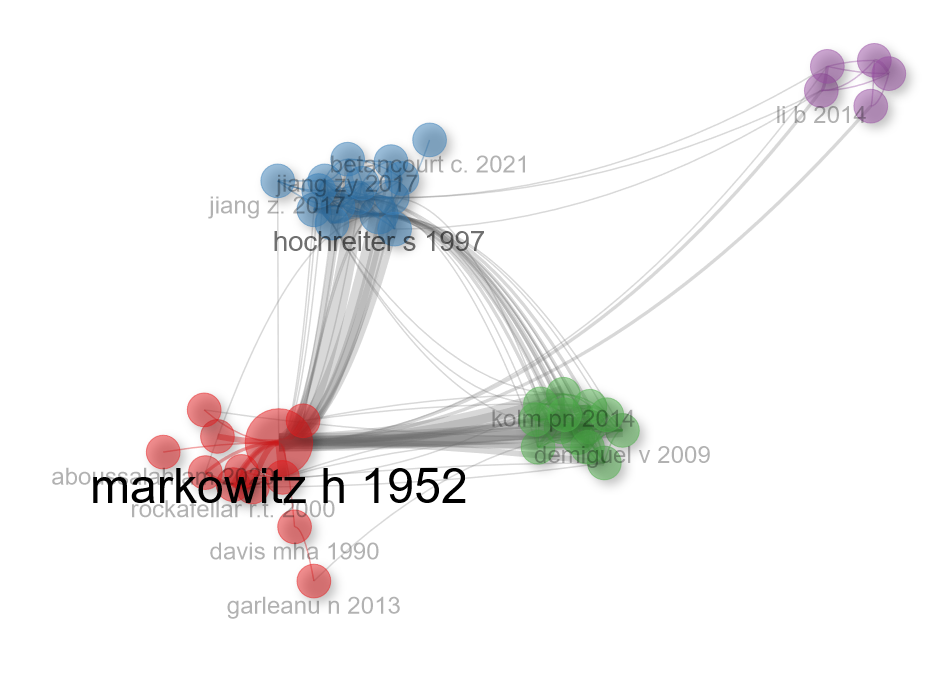
\includegraphics[width=0.98\textwidth]{./images/cocitation_network.png}
                    \par \footnotesize Fonte: próprio autor.
                \end{figure}

            \end{column}
        \end{columns}
        


    \end{frame}
    \note{Co-citação e referencias mais citadas}
%-------------------------------------------------------





%-------------------------------------------------------
    \begin{frame}{Risco e Retorno}

        \LARGE

        \begin{equation}
            \text{Retorno} = \frac{{P_f-P_i}}{{P_i}}
        \end{equation}

        % side by side text and figure
        \begin{columns}
            \begin{column}{0.3\textwidth}


                Retorno esperado:
                \begin{itemize}
                    \item Média
                    \item Média Móvel
                    \item Média Móvel Exponencial
                    \item Outros
                \end{itemize}

            \end{column}
            \begin{column}{0.3\textwidth}

                Risco:
                \begin{itemize}
                    \item Variância
                    \item Desvio Padrão
                    \item GARCH
                \end{itemize}

                \vspace{25pt}

            \end{column}

            \begin{column}{0.3\textwidth}

                Portfólio:
                \begin{itemize}
                    \item Média ponderada
                    \item Matriz de Covariância
                \end{itemize}

                \vspace{25pt}

            \end{column}
        \end{columns}
                

    \end{frame}
    \note{Média e variância}
%-------------------------------------------------------




%-------------------------------------------------------
    \begin{frame}{Otimização de Portfólio}


        \LARGE \textbf{Média e Variância}

        % side by side text and figure
        \begin{columns}
            \begin{column}{0.5\textwidth}

                \begin{equation}
                    \label{eq:markowitz}
                    \begin{aligned}
                        & \underset{w}{\text{minimizar}}
                        & & w^T \Sigma w \\
                        & \text{sujeito a}
                        & & w^T \mu = \mu_p \\
                        & & & w^T \mathbf{1} = 1 \\
                        & & & w \geq 0
                    \end{aligned}
                \end{equation}
        
            \end{column}
            \begin{column}{0.5\textwidth}

                \begin{figure}[htbp]
                    \centering
                    \caption{Otimização de portfólio utilizando o modelo de média-variância}
                    \label{fig:mínimo_risco}
                    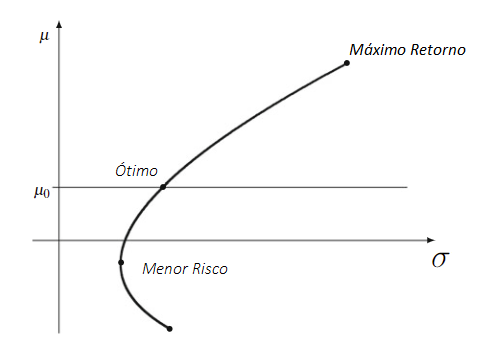
\includegraphics[width=0.6\textwidth]{images/minimo_risco.png}
                    \par \footnotesize Fonte: adaptado de \citeauthor{mansini2015linear}.
                \end{figure}
        
            \end{column}
        \end{columns}
        

    \end{frame}
    \note{Média e variância, Sharpe}
%-------------------------------------------------------





%-------------------------------------------------------
    \begin{frame}{Otimização de Portfólio}

        \LARGE \textbf{Aversão ao Risco}

        % side by side text and figure
        \begin{columns}
            \begin{column}{0.5\textwidth}

                \begin{equation}
                    \label{eq:aversao}
                    \begin{aligned}
                        & \underset{w}{\text{maximizar}}
                        & & w^T \mu - \lambda w^T \Sigma w \\
                        & \text{sujeito a} \\
                        & & & w^T \mathbf{1} = 1 \\
                        & & & w \geq 0
                    \end{aligned}
                \end{equation}
            \end{column}

            \begin{column}{0.5\textwidth}

                \begin{figure}[htbp]
                    \centering
                    \caption{Otimização de portfólio utilizando o modelo com o parâmetro $\lambda$ de aversão ao risco}
                    \label{fig:aversao}
                    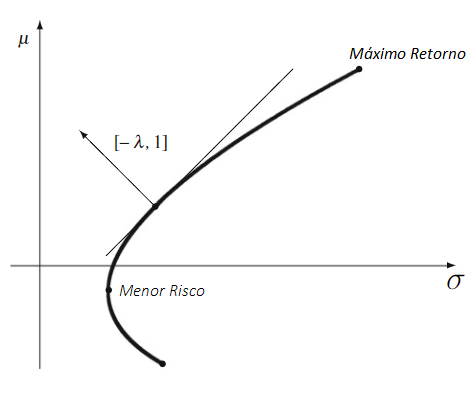
\includegraphics[width=0.6\textwidth]{images/aversao.png}
                    \par \footnotesize Fonte: adaptado de \citeauthor{mansini2015linear}.
                \end{figure}
        
            \end{column}
        \end{columns}

    \end{frame}
    \note{Outros modelos, restrições reais e heurística}
%-------------------------------------------------------




%-------------------------------------------------------
    \begin{frame}{Otimização de Portfólio}

        \LARGE \textbf{Maximização do Índice de Sharpe}

        % side by side text and figure
        \begin{columns}
            \begin{column}{0.5\textwidth}

                \begin{equation}
                    \label{eq:sharpe}
                    \begin{aligned}
                        & \underset{w}{\text{maximizar}}
                        & & \frac{w^T \mu - r_f}{\sqrt{w^T \Sigma w}} \\
                        & \text{sujeito a} \\
                        & & & w^T \mathbf{1} = 1 \\
                        & & & w \geq 0
                    \end{aligned}
                \end{equation}

            \end{column}

            \begin{column}{0.5\textwidth}

                    \begin{figure}[htbp]
                        \centering
                        \caption{Linha do mercado de capitais}
                        \label{fig:carteira_de_mercado}
                        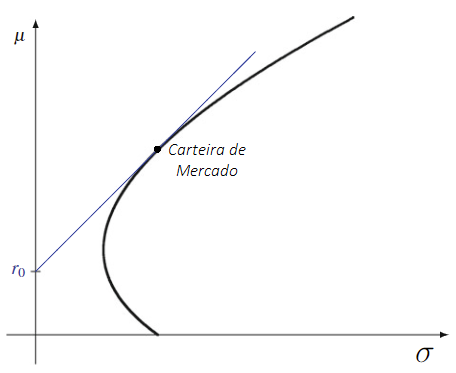
\includegraphics[width=0.6\textwidth]{images/carteira_de_mercado.png}
                        \par \footnotesize Fonte: adaptado de \citeauthor{mansini2015linear}.
                    \end{figure}
        
            \end{column}
        \end{columns}

    \end{frame}
    \note{Outros modelos, restrições reais e heurística}
%-------------------------------------------------------





%-------------------------------------------------------
    \begin{frame}{Otimização de Portfólio}

        \LARGE \textbf{Parâmetros Reais}

        \begin{itemize}
            \item Restrições de capital de investimento
            \item Custos de operação
            \item Cotação e lotes de negociação
            \item Rebalanceamento
            \item Cardinealidade
            \item Aversão ao risco
        \end{itemize}

        Problema de otimização não linear inteiro misto, NP-difícil.

    \end{frame}
    \note{Outros modelos, restrições reais e heurística}
%-------------------------------------------------------




%-------------------------------------------------------
    \begin{frame}{Redes Neurais}

        As Redes Neurais são modelos computacionais inspirados no funcionamento do cérebro humano, capazes de aprender e realizar tarefas complexas de processamento de informações.

        \begin{figure}[htbp]
            \centering
            \caption{Célula LSTM.}
            \label{fig:lstm}
            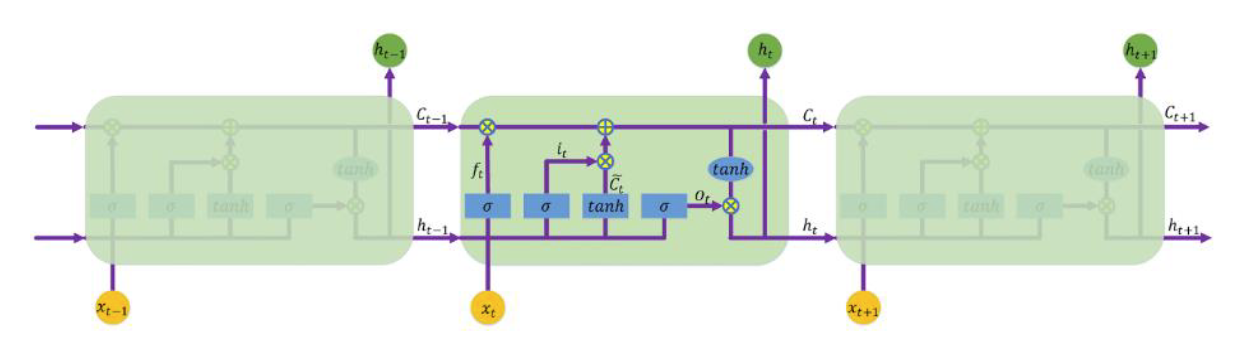
\includegraphics[width=0.95\textwidth]{images/lstm.png}
            \par \footnotesize Fonte: \citeauthor{ta2020portfolio}.
        \end{figure}


    \end{frame}
    \note{Principais métodos}
%-------------------------------------------------------





%-------------------------------------------------------
    \begin{frame}{Redes Neurais Recorrentes e Atenção}

        \Large
        % side by side text and figure
        \begin{columns}
            \begin{column}{0.5\textwidth}

                Mecanismo de atenção é capaz de capturar dependências de longo alcance entre origem e destino. Modelos:

                \begin{itemize}
                    \item Atenção Aditiva (\citeauthor{bahdanau2015neural})
                    \item Auto Atenção (\citeauthor{vaswani2017attention})
                \end{itemize}
                

            \end{column}

            \begin{column}{0.5\textwidth}

                \begin{figure}[htbp]
                    \centering
                    \caption{Mecanismo de atenção.}
                    \label{fig:attention}
                    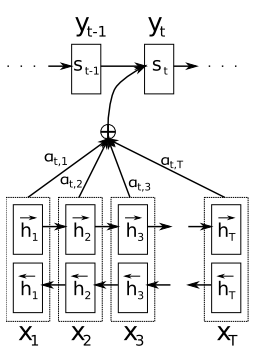
\includegraphics[width=0.5\textwidth]{images/attention.png}
                    \par \footnotesize Fonte: \citeauthor{bahdanau2015neural}.
                \end{figure}
        
        
            \end{column}
        \end{columns}


    \end{frame}
    \note{Arquitura e atenção}
%-------------------------------------------------------


    %-------------------------------------------------------
\section{Metodologia}
%-------------------------------------------------------



%-------------------------------------------------------
    \begin{frame}{Etapas}

        \LARGE

        A metodologia está dividida em algumas etapas:

        \begin{enumerate}
            \item Coleta de dados
            \item Pré-processamento
            \item Modelagem de dados
            \item Otimização de portfólio
            \item Treinamento de redes neurais 
            \item Validação de modelos
        \end{enumerate}

    \end{frame}
    \note{Metodologia}
%-------------------------------------------------------




%-------------------------------------------------------
    \begin{frame}{Coleta de dados}

        \begin{quadro}[htp]
            \centering
            \caption{Dados coletados}
            \label{quadro:coleta_dados}
            \resizebox{.7\columnwidth}{!}{%
            \begin{tabular}{lll}
                \hline
                \textbf{Dados} & \textbf{Fonte} & \textbf{Descrição} \\ \hline \hline
                Preços de ativos & B3 & \begin{tabular}[c]{@{}l@{}}Preços diário de ativos financeiros \\ negociados na B3\end{tabular} \\ \hline
                Índice Bovespa & B3 & \begin{tabular}[c]{@{}l@{}}Índice de mercado diário calculado \\ pela B3\end{tabular} \\ \hline
                Componentes do Ibovespa & B3 & \begin{tabular}[c]{@{}l@{}}Lista de ativos financeiros componentes \\ do Ibovespa\end{tabular} \\ \hline
                Informações cadastrais de ativos & B3 & \begin{tabular}[c]{@{}l@{}}Informações cadastrais no dia dos ativos \\ financeiros listados na B3 \end{tabular} \\ \hline
                Taxa SELIC & Banco Central & \begin{tabular}[c]{@{}l@{}}Taxa de juros anual por dia pelo Banco \\ Central\end{tabular} \\ \hline
                Taxas de corretagem & Corretora & \begin{tabular}[c]{@{}l@{}}Taxas de corretagem cobradas pelas\\ corretoras\end{tabular} \\ \hline
                Taxas de custódia & Corretora & \begin{tabular}[c]{@{}l@{}}Taxas de custódia cobradas pela B3 \\ \end{tabular} \\ \hline
                Imposto de renda & Receita Federal & \begin{tabular}[c]{@{}l@{}}Tabela de alíquotas de imposto de renda \\ por tipo de ativo\end{tabular} \\ \hline
                Desdobramentos e grupamentos & \textit{Yahoo Finance} & \begin{tabular}[c]{@{}l@{}}Desdobramentos e grupamentos de \\ ativos financeiros\end{tabular} \\ \hline
            \end{tabular}%
            }
            \par \footnotesize Fonte: próprio autor.
        \end{quadro} 
        
    \end{frame}
    \note{Tabela com fontes}
%-------------------------------------------------------



%-------------------------------------------------------
    \begin{frame}{Pré-processamento}

        \begin{figure}[htp]
            \centering
            \caption{Fluxo de pré-processamento de dados}
            \label{fig:fluxo_preprocessamento}
            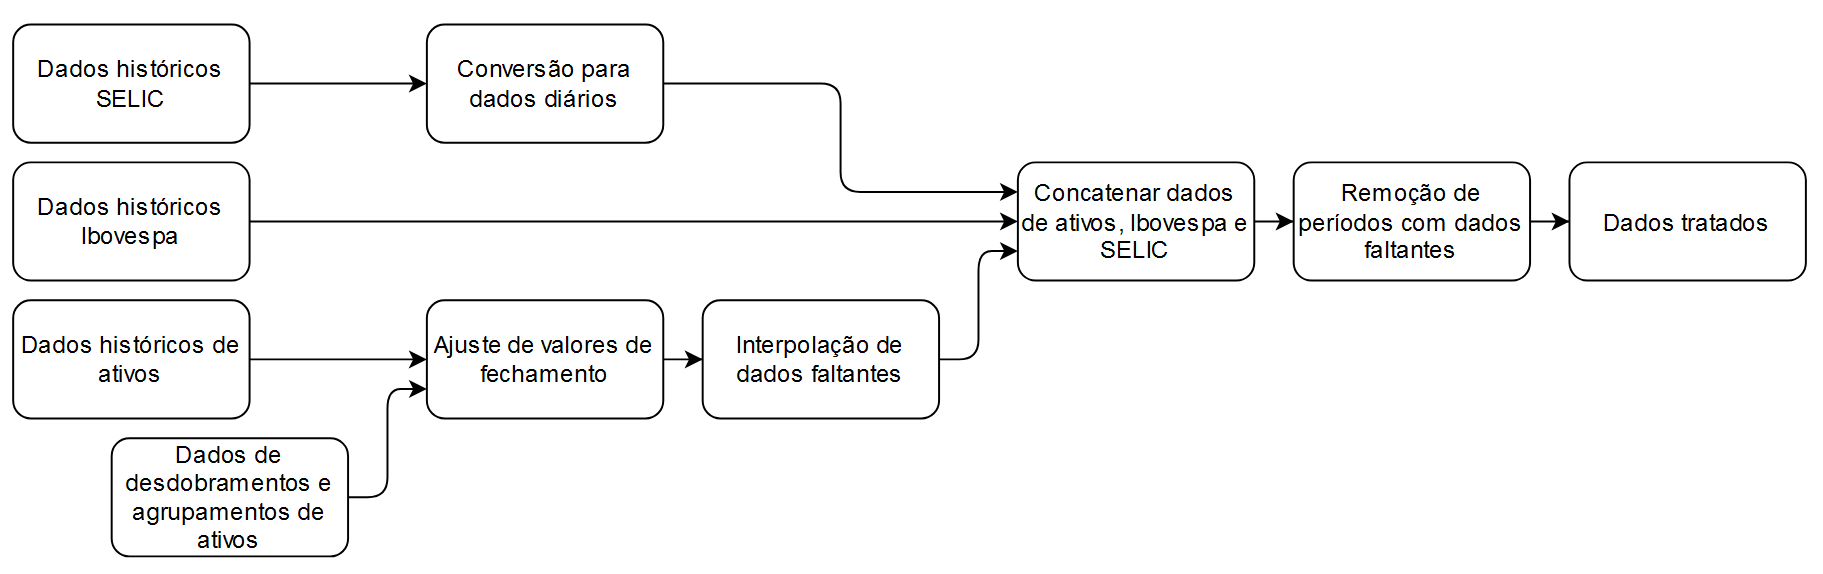
\includegraphics[width=\textwidth]{images/fluxo_tratamento.png}
            \par \footnotesize Fonte: próprio autor.
        \end{figure}
        
    \end{frame}
    \note{Fluxo pré-processamento}
%-------------------------------------------------------




%-------------------------------------------------------
    \begin{frame}{Modelagem}

        \Large

        Desenvolvido módulo onde são preparadas as seguintes combinações.

        \begin{itemize}
            \item Intervalos de tempo: diários, semanais e mensais
            \item Métodos de cálculo de retorno: média simples, médias móveis, médias móveis exponenciais e ARIMA(0,1,1)
            \item Métodos de cálculo de risco: desvio padrão e GARCH(1,1)
        \end{itemize}

        Como exemplo, filtra-se dados de início de semana a partir de 2018 por 60 semanas. Os dados são agrupados por semana, ou seja, o primeiro dia da semana será a referência para o filtro dos dados. Em seguida, são selecionados os valores das datas obtidas, e calcula-se o retorno médio e o desvio padrão dos retornos.
        
    \end{frame}
    \note{Parâmetros, arquitetura}
%-------------------------------------------------------




%-------------------------------------------------------
    \begin{frame}{Otimização de Portfólio}

        \Large

        Modelo proposto a aplicação das seguintes restrições: capital de investimento, custos de operação, cotação e lotes de negociação, rebalanceamento, aversão ao risco e somente posições de compra. 
        
        Este modelo permite responder as seguintes perguntas: quanto dinheiro tem, e quanto aceita perder no intervalo de investimento para obter o máximo retorno?
        
        $\kappa_{j}$ é a variável de decisão, $\delta_{j}$ e $z_{j}$ são as variáveis auxiliares. A descrição segue:
        
        \begin{equation*}
            \begin{aligned}
                \kappa_{j}  \geq 0 \ \in \mathbb{Z} \quad j=1, \ldots, n , \quad & \text{quantidade de lotes} \\
                \delta_{j}  \geq 0 \ \in \mathbb{Z} \quad j=1, \ldots, n , \quad & \text{quantidade de rebalanceamento no lote} \\
                z_{j} \in\{0,1\} \quad j=1, \ldots, n, \quad & \text{1 se o ativo alterar quantidade}
            \end{aligned}
        \end{equation*}

    \end{frame}
    \note{Modelo e restrições}
%-------------------------------------------------------





%-------------------------------------------------------
    \begin{frame}{Otimização de Portfólio}

        Função objetivo, variáveis dependentes, cotação e lotes de negociação:

        \begin{columns}
            \begin{column}{0.5\textwidth}

                \begin{subequations}
                    \label{eq:otimizacao_1}
                    \begin{align}
                        % 
                        & \underset{\kappa}{\text{maximizar}}
                        & & \frac{r_{p}(\kappa) - \frac{r_{f}}{(1+c_{r_{f}}) C_{p}(\kappa)}}{\sigma_{p}(\kappa)} \\
                        % 
                        & \text{sujeito a} \notag \\
                        % 
                        & & & r_{p}(\kappa) = \sum_{j=1}^{n} \kappa_{j} q_{j} \mu_{j} -  \sum_{j=1}^{n} K_{j} \\
                        % 
                        & & & \sigma_{p}(\kappa) = \sqrt{\sum_{j=1}^{n} \sum_{i=1}^{n} \kappa_{j} \kappa_{i} q_{j} q_{i} \sigma_{j} \sigma_{i} \rho_{ij}} \\
                        % 
                        & & & C_{p}(\kappa) = \sum_{j=1}^{n} q_{j}\kappa_{j} + K_{j}
                        % 
                    \end{align}
                \end{subequations}
            \end{column}

            \begin{column}{0.5\textwidth}

                \begin{equation*}
                    \begin{aligned}
                        r_{p} : \quad & \text{retorno da carteira} \\
                        \sigma_{p} : \quad & \text{risco da carteira} \\
                        r_{f} : \quad & \text{retorno livre de risco} \\
                        C_{p} : \quad & \text{capital da carteira} \\
                        c_{r_{f}} : \quad & \text{taxa de imposto para ativo livre de risco} \\
                        q_{j} : \quad & \text{cotação do lote padrão} \\
                        K_{j} : \quad & \text{custo de transação do ativo}
                    \end{aligned}
                \end{equation*}

            \end{column}
        \end{columns}




    \end{frame}
    \note{Restrições reais}
%-------------------------------------------------------






%-------------------------------------------------------
    \begin{frame}{Otimização de Portfólio}

        Restrições de capital, custos de operação e rebalanceamento:

        \begin{columns}
            \begin{column}{0.5\textwidth}

                \begin{subequations}
                    \label{eq:otimizacao_2}
                    \begin{align}
                        & K_{j} = \sum_{j=1}^{n}c_{j}q_{j}\delta_{j} + \sum_{j=1}^{n} f_{j} z_{j}   \\
                        %
                        & C_{0} = \sum_{i=1}^{n}q_{i}\kappa_{i}^{0}+ B \\
                        %
                        & C_{0} \geq C_{p} \\
                        % 
                        &  q_{j}\kappa_{j} \leq z_{j} C_{0} \quad j=1, \ldots, n \text{,} \\
                        % 
                        & \delta_{j} \geq \left( \kappa_{j} -\kappa_{j}^{0} \right) \quad j=1, \ldots, n \\
                        % 
                        & \delta_{j} \geq -\left( \kappa_{j} -\kappa_{j}^{0} \right) \quad j=1, \ldots, n \\
                        % 
                        & \delta_{j} \leq \gamma_{j}z_{j} \quad j=1, \ldots, n
                    \end{align}
                \end{subequations}
            \end{column}

            \begin{column}{0.5\textwidth}

                \begin{equation*}
                    \begin{aligned}
                        f_{j} : \quad & \text{taxa de transação do ativo} \\
                        c_{j} : \quad & \text{custo de transação do ativo} \\
                        \kappa_{j}^{0} : \quad & \text{quantidade inicial de lotes do ativo} \\
                        \gamma_{j} : \quad & \text{quantidade máxima de lotes do ativo}
                    \end{aligned}
                \end{equation*}

            \end{column}
        \end{columns}

    \end{frame}
    \note{Otimizadores}
%-------------------------------------------------------







%-------------------------------------------------------
    \begin{frame}{Otimização de Portfólio}

        Restrições de aversão ao risco:

        \begin{columns}
            \begin{column}{0.5\textwidth}


                \begin{subequations}
                    \label{eq:otimizacao_4}
                    \begin{align}
                        & r_{inv} - \sigma_{inv} Z_{\beta} \geq VaR \\
                        % 
                        & \sigma_{inv} = \sigma_{p} \frac{C_{p}}{C_{0}} \\
                        % 
                        & r_{inv} = \frac{C_{0} - C_{p}}{C_{0}} \frac{r_{f}}{(1+c_{r_{f}})} + \frac{C_{p}}{C_{0}} r_{p}
                    \end{align}
                \end{subequations}

            \end{column}

            \begin{column}{0.5\textwidth}

                \begin{equation*}
                    \begin{aligned}
                        r_{inv} : \quad & \text{retorno do investimento} \\
                        \sigma_{inv} : \quad & \text{risco do investimento} \\
                        VaR : \quad & \text{valor monetário aceitável de perda} \\
                        Z_{\beta} : \quad & \text{quantil da distribuição normal padrão} \\
                        & \quad \text{ ao nível de confiança }\beta.
                    \end{aligned}
                \end{equation*}

            \end{column}
        \end{columns}

    \end{frame}
    \note{Otimizadores}
%-------------------------------------------------------


%-------------------------------------------------------
    \begin{frame}{Otimização de Portfólio}

        \LARGE
        Métodos para otimização:

        \begin{itemize}
            \item Otimização de portfólio sem restrições reais: SLSQP (\citeauthor{kraft1988sqlsp})
            \item Otimização de portfólio com restrições: APOPT (\citeauthor{hedengren2014nonlinear}).
            \item Inicialização do otimizador: Distribuição Dirichlet \cite{yang2022selective}.
            \item Matheurística:  Busca no núcleo (\citeauthor{angelelli2012kernel}).
        \end{itemize}

        
    \end{frame}
    \note{Heurística}
%-------------------------------------------------------





%-------------------------------------------------------
    \begin{frame}{Treinamento de redes neurais}


        
        \begin{columns}
            \begin{column}{0.5\textwidth}

                \begin{figure}[htp]
                    \centering
                    \caption{Fluxograma de redes neurais de RNN com auto atenção.}
                    \label{fig:RNN_SelfAtt}
                    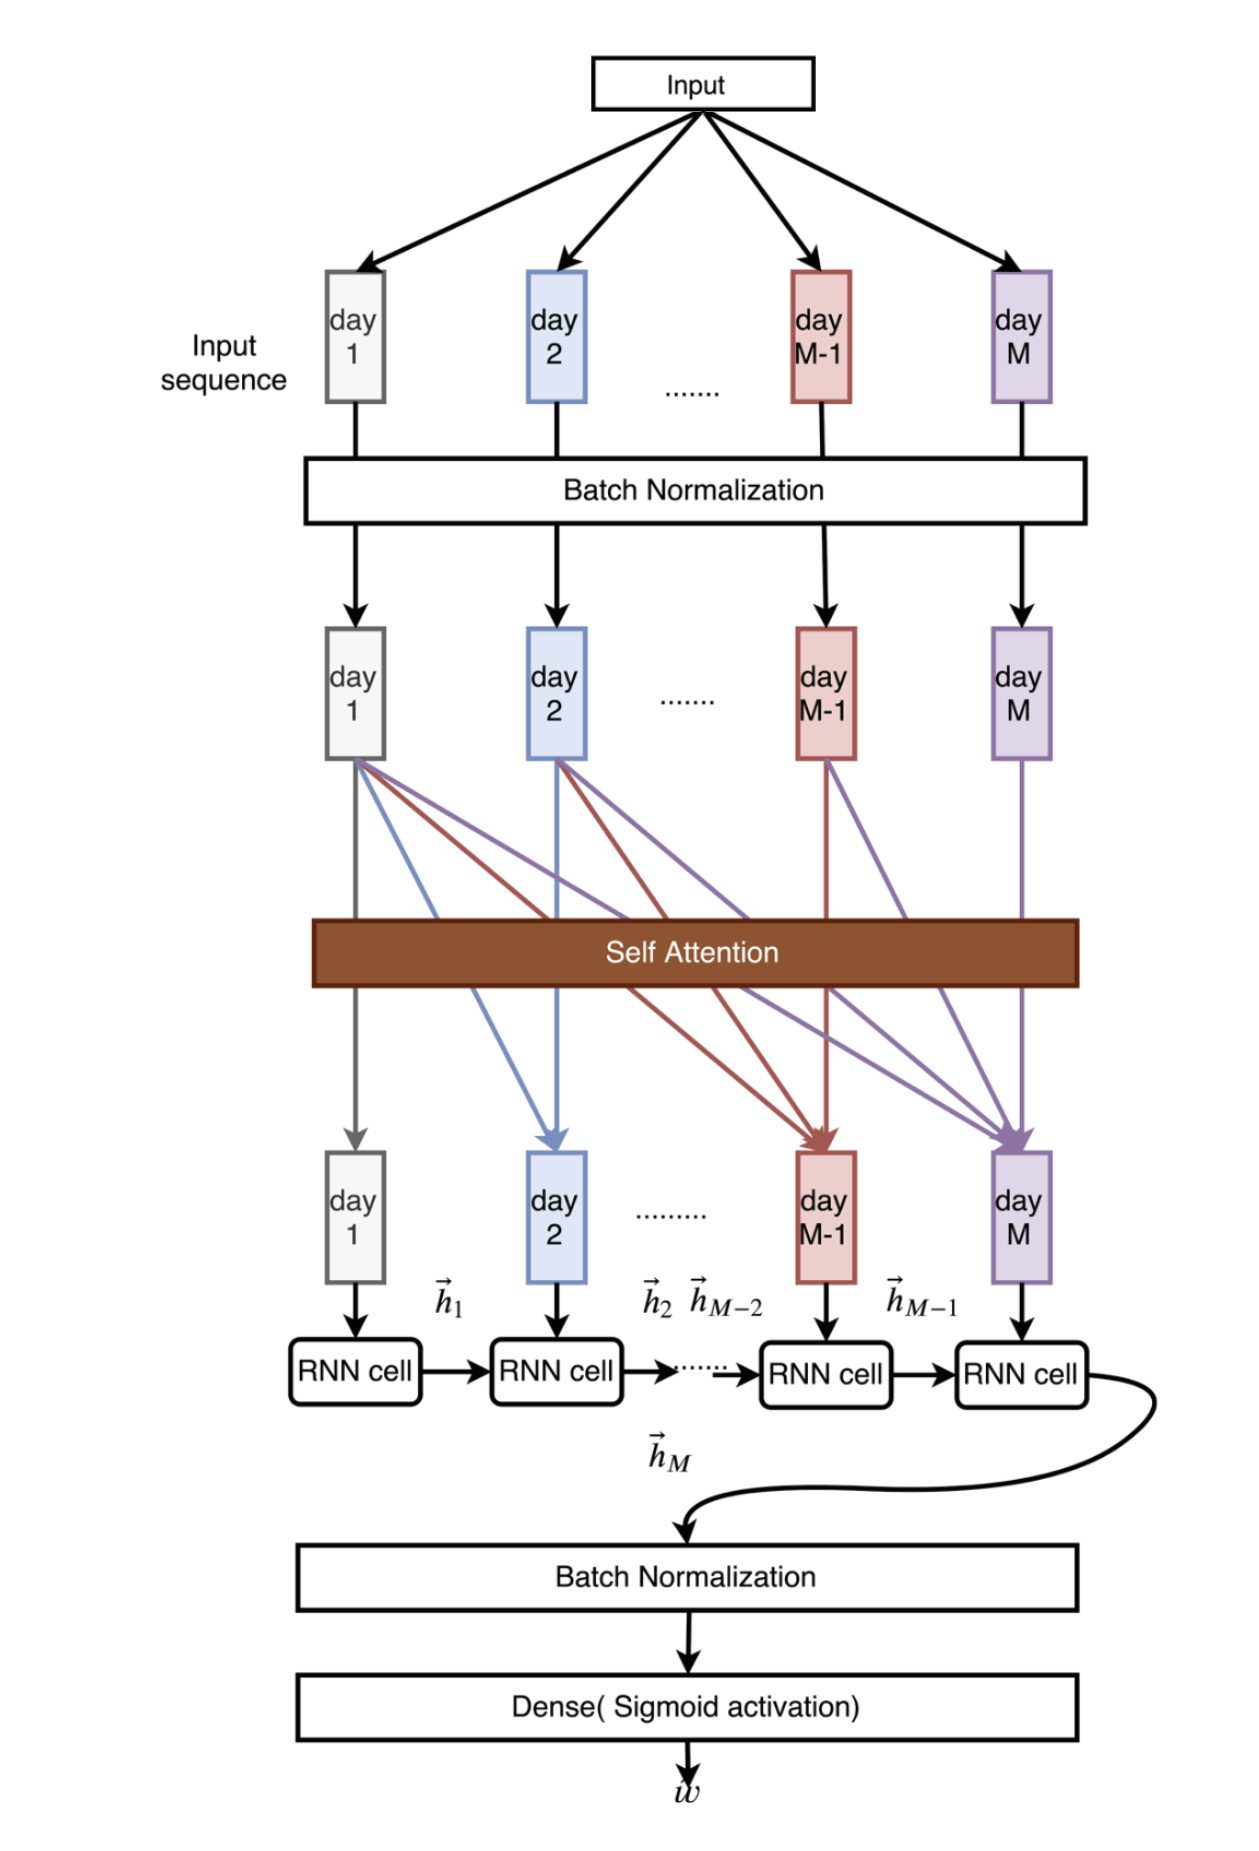
\includegraphics[width=0.55\textwidth]{./images/RNN_SelfAtt.png}
                    \par \footnotesize Fonte: adaptado de \citeauthor{cao2020delafo}.
                \end{figure}


            \end{column}

            \begin{column}{0.5\textwidth}

                \begin{figure}[htp]
                    \centering
                    \caption{Estrutura de rede neural LSTM com auto atenção.}
                    \label{fig:model_lstm_SelfAtt}
                    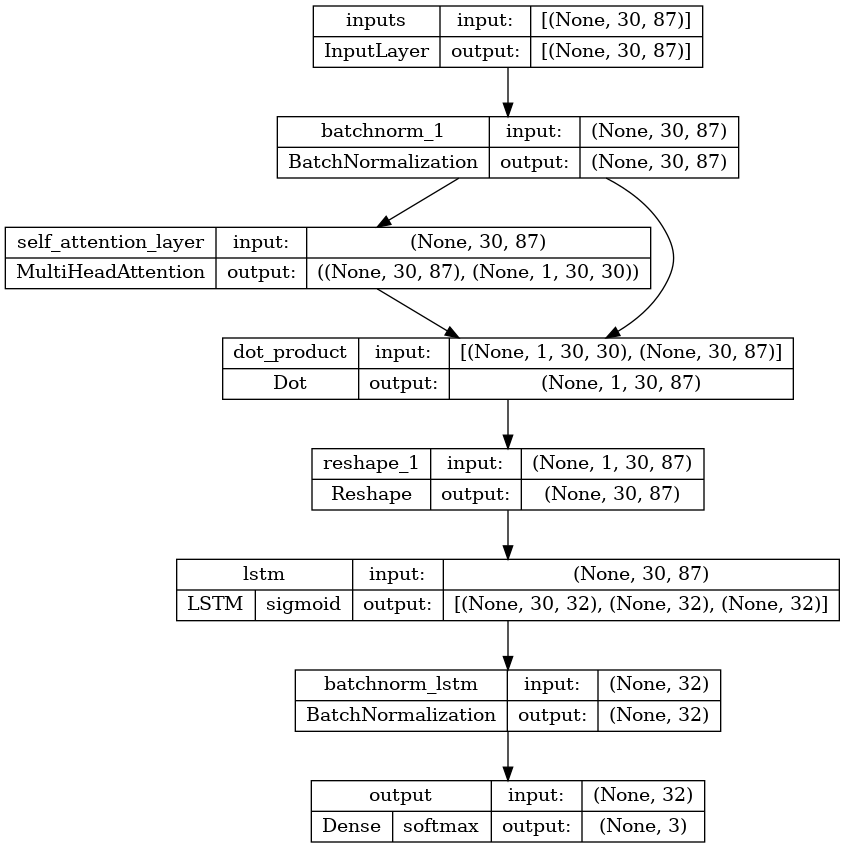
\includegraphics[width=0.65\textwidth]{./images/lstm_selfatt.png}
                    \par \footnotesize Fonte: próprio autor.
                \end{figure}

            \end{column}
        \end{columns}

        
    \end{frame}
    \note{Estruturas de redes RNN e Auto Atenção}
%-------------------------------------------------------




%-------------------------------------------------------
    \begin{frame}{Treinamento de redes neurais}

        
        \begin{columns}
            \begin{column}{0.5\textwidth}

                \begin{figure}[htp]
                    \centering
                    \caption{Fluxograma de redes neurais de RNN com atenção de Bahdanau.}
                    \label{fig:RNN_BauhAtt}
                    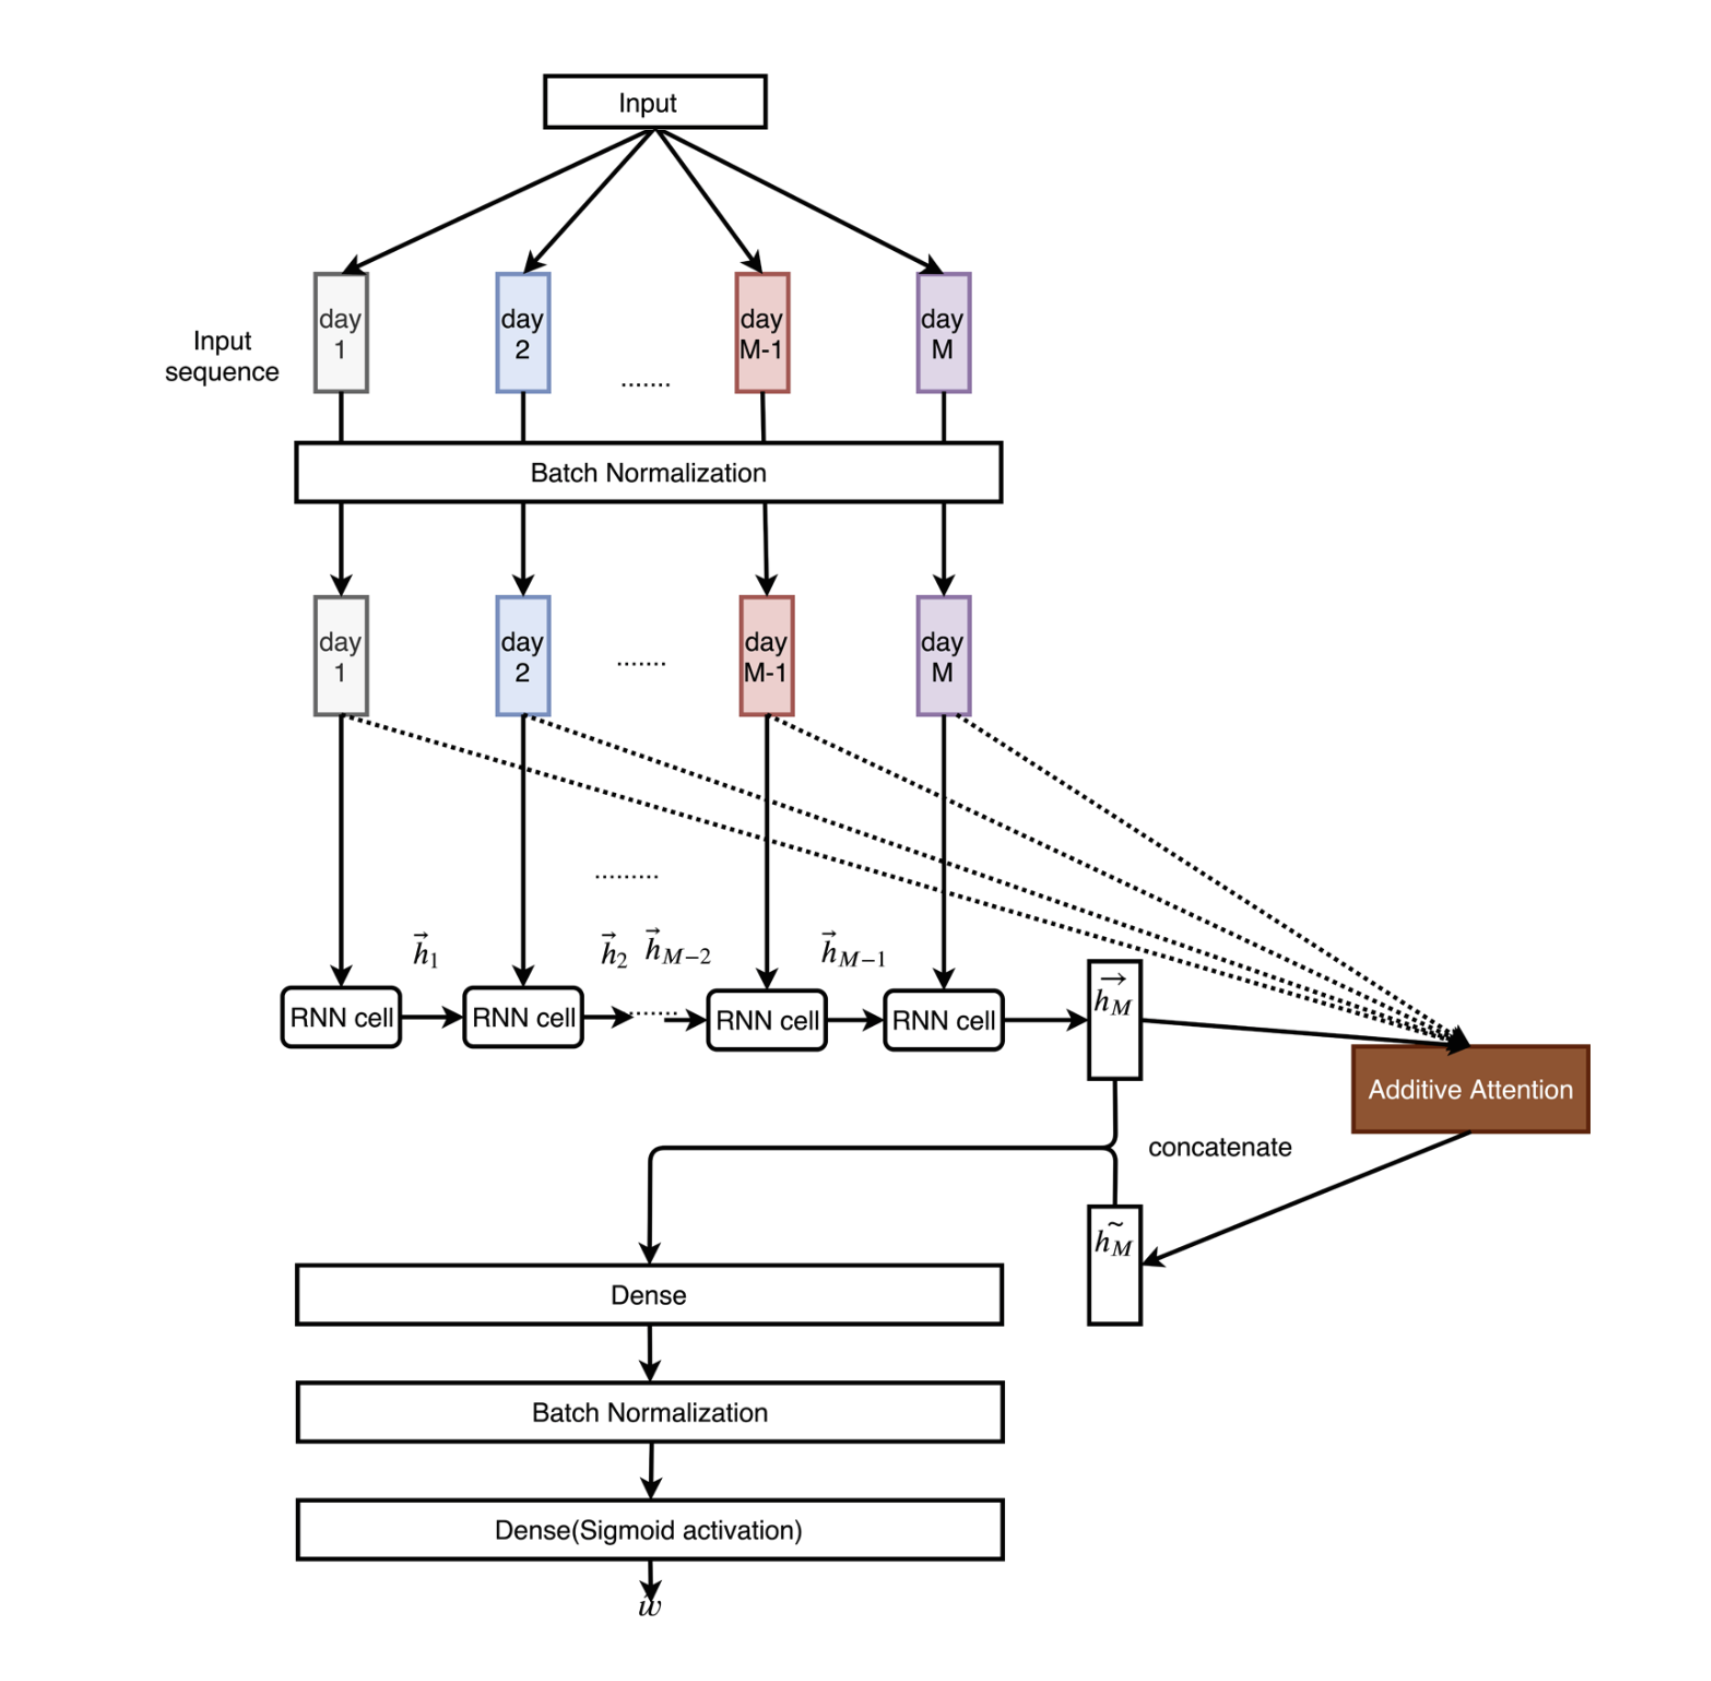
\includegraphics[width=0.8\textwidth]{./images/RNN_AddAtt.png}
                    \par \footnotesize Fonte: adaptado de \citeauthor{cao2020delafo}.
                \end{figure}

            \end{column}

            \begin{column}{0.5\textwidth}

                \begin{figure}[htpb]
                    \centering
                    \caption{Estrutura de rede neural LSTM com atenção de Bahdanau.}
                    \label{fig:model_lstm_BauhAtt}
                    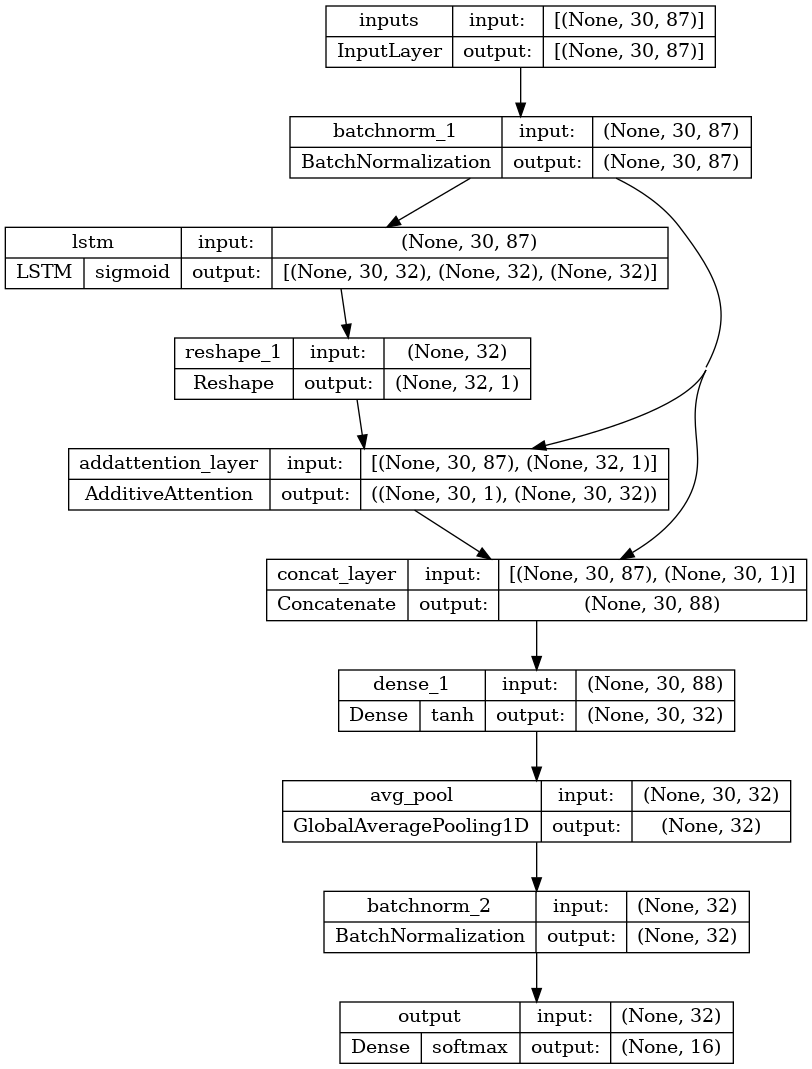
\includegraphics[width=0.6\textwidth]{./images/model_lstm_BauhAtt.png}
                    \par \footnotesize Fonte: próprio autor.
                \end{figure}

            \end{column}
        \end{columns}

        
    \end{frame}
    \note{Estruturas de redes RNN e Atenção de Bahdanau}
%-------------------------------------------------------





%-------------------------------------------------------
    \begin{frame}{Treinamento de redes neurais}


        \begin{columns}
            \begin{column}{0.5\textwidth}

                Período de análise: 09/2018 - 01/2023

                Hiperparâmetros: Hyperband Tuning,

                \begin{itemize}
                    \item Taxa de aprendizagem: $0.0001$ a $1$ distribuídos em função logarítmica reversa.
                    \item Regularização $L_{2}$: $0.0001$ a $1$ distribuídos em função logarítmica reversa.
                    \item Épocas: 30.
                \end{itemize}

                Validação cruzada: 10 \textit{folds} com lacunas de duas partes anteriores e uma parte posterior.

                
                Função de perda: entropia cruzada categórica.
                
                Métrica: acurácia.

            \end{column}

            \begin{column}{0.5\textwidth}


                \begin{figure}[htp]
                    \centering
                    \caption{Validação cruzada com lacunas.}
                    \label{fig:cross_validation}
                    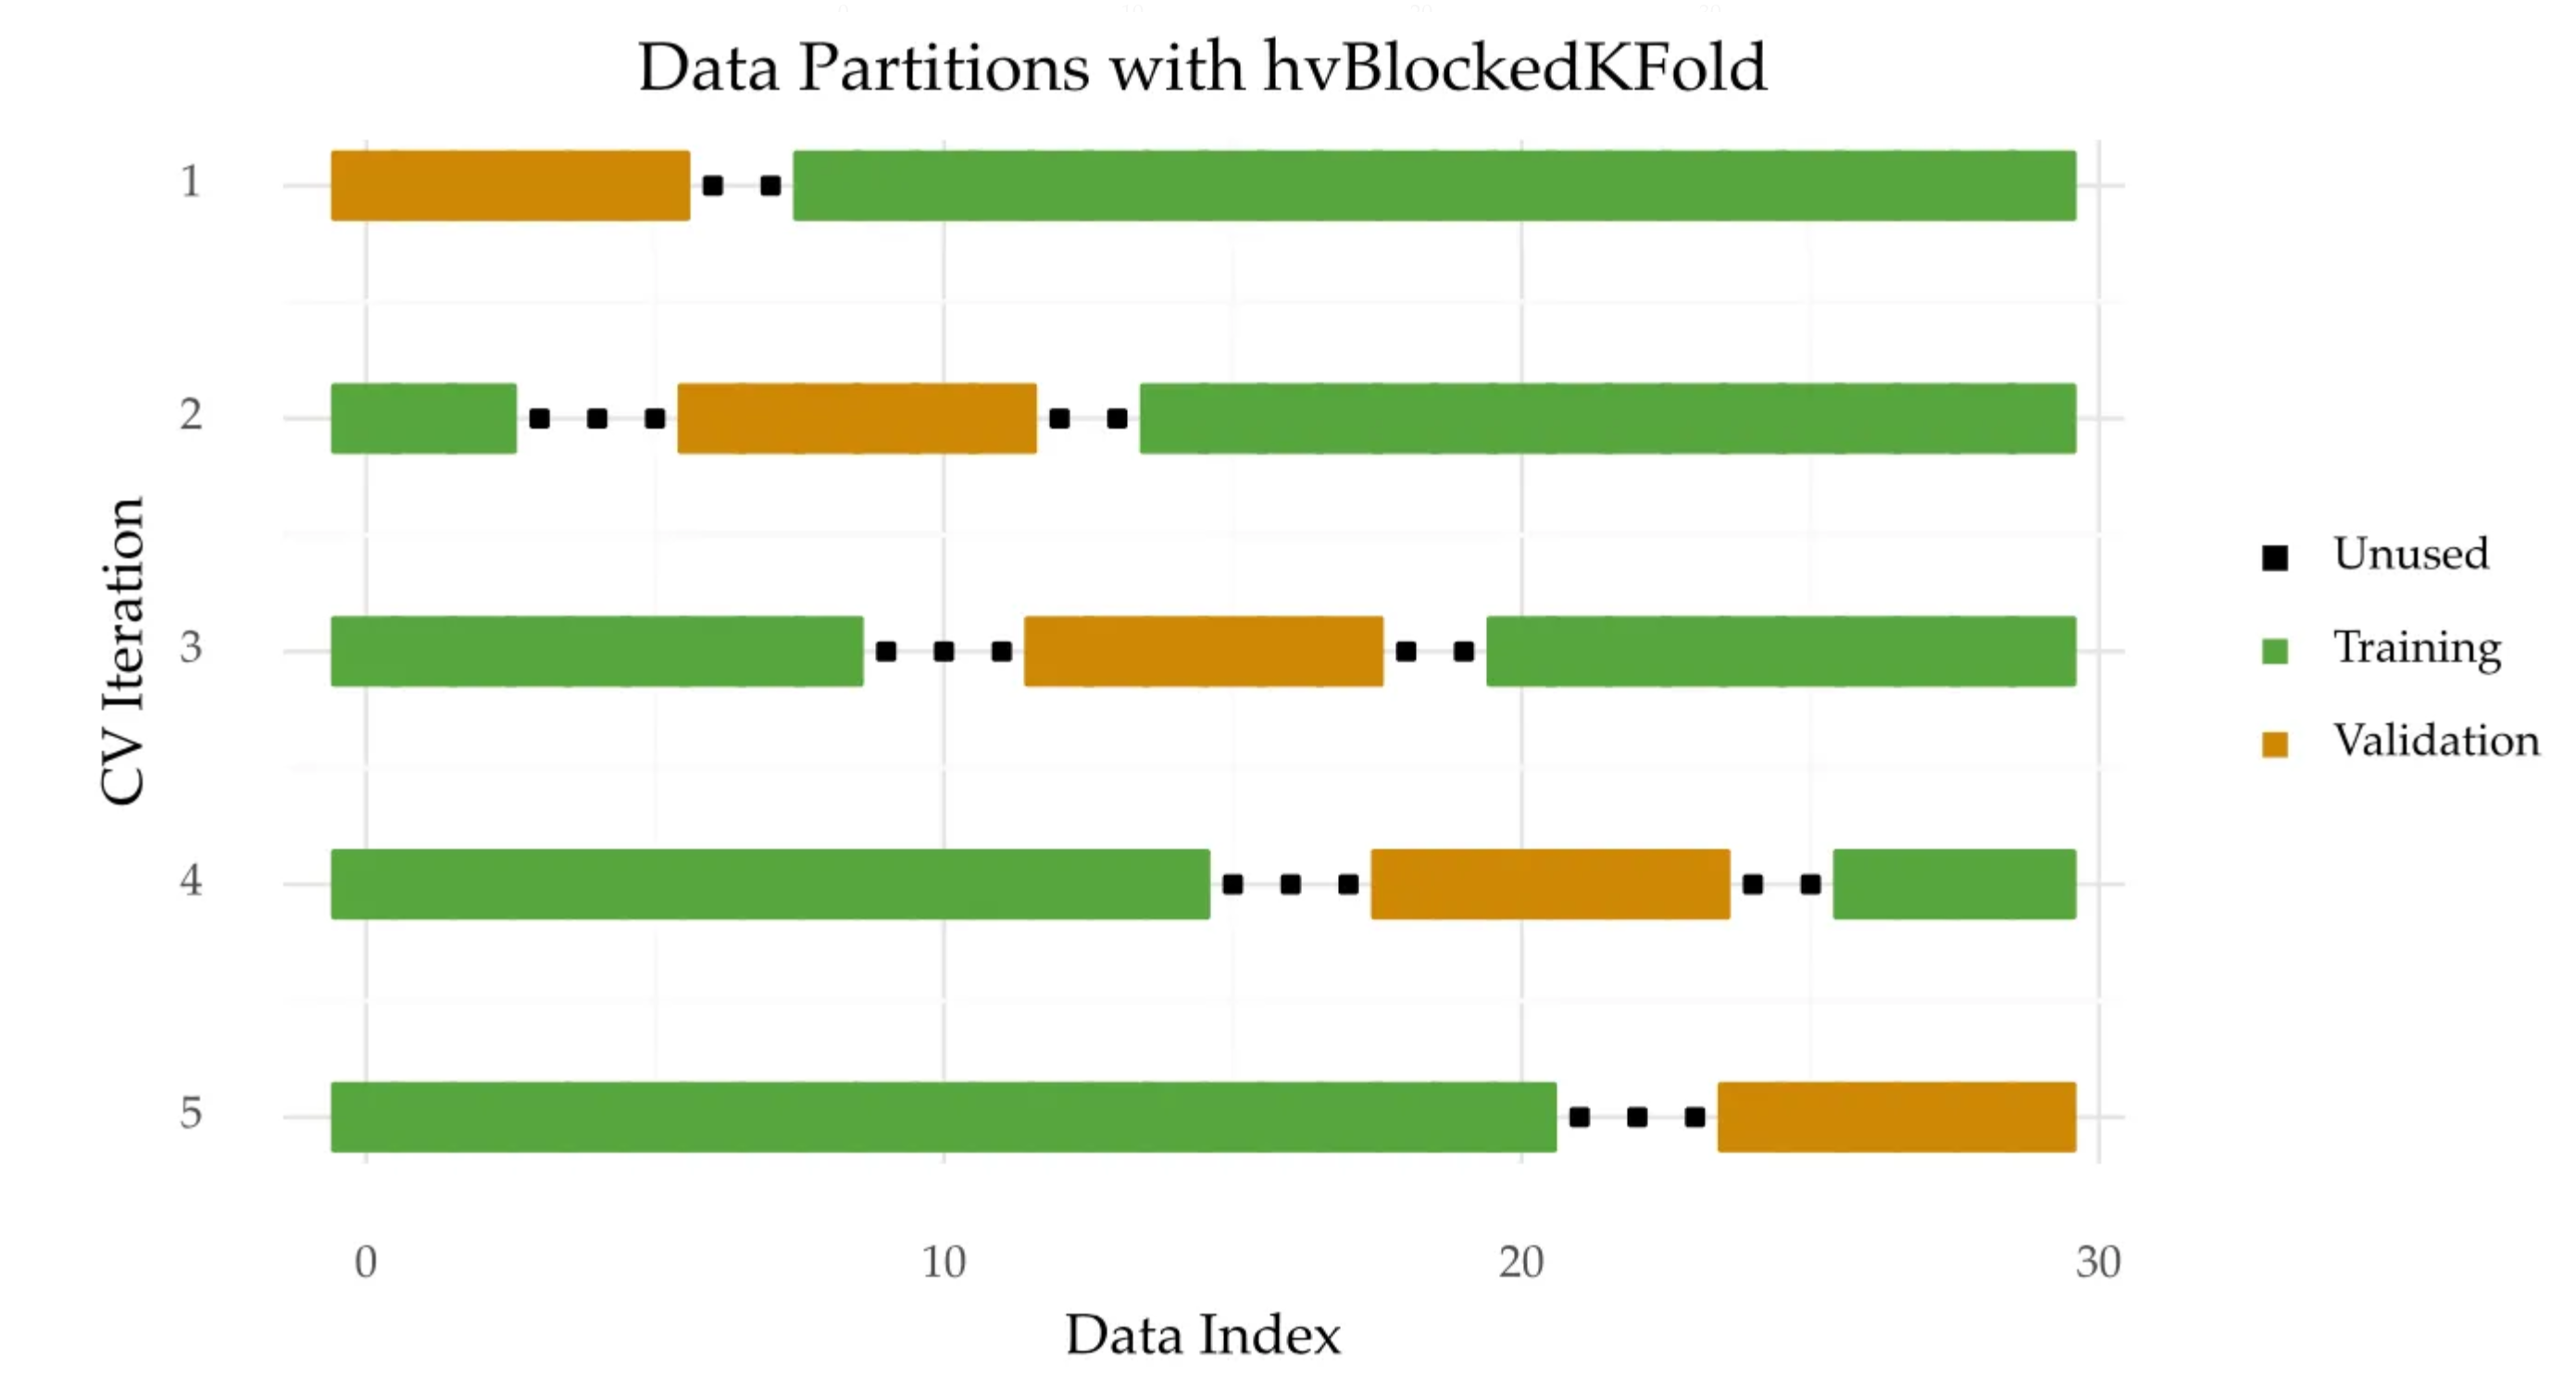
\includegraphics[width=0.8\textwidth]{./images/cross_validation.png}
                    \par \footnotesize Fonte: \citeauthor{Cerqueira2023}.
                \end{figure}

            \end{column}
        \end{columns}

    \end{frame}
    \note{Hiperparâmetros, e separação dos dados}
%-------------------------------------------------------




%-------------------------------------------------------
    \begin{frame}{Validação de redes neurais}

        Período de análise: 09/2018 - 07/2023

        Dados de entrada: bloco dos últimos 30 dias de preços de fechamento ajustado de 87 ativos do Ibovespa.

        Divisão dos dados:

        \begin{itemize}
            \item 90\% para treinamento (validação cruzada), 1078 amostras.
            \item 10\% para teste, 120 amostras.
        \end{itemize}

        Atributos alvo: melhor carteira no próximo período dentre 3 carteiras otimizadas pelo índice Sharpe.

        \begin{itemize}
            \item Parâmetros de modelagem: média simples e desvio padrão.
            \item Intervalo de tempo para retorno: últimos 15, 30 e 60 dias.
            \item Intervalo de ajuste da otimização: diário.
        \end{itemize}
        
    \end{frame}
    \note{Cross validation e métricas}
%-------------------------------------------------------


    
%-------------------------------------------------------
\section{Resultados}
%-------------------------------------------------------

%-------------------------------------------------------
    \begin{frame}{Otimização com Parâmetros Reais}
        No cálculo foram considerados média e desvio padrão dos últimos 30 dias e risco igual a taxa SELIC para o último dia de junho de 2023.

            \begin{figure}[H]
                \centering
                \caption{Evolução da convergência de otimização da carteira}
                \label{fig:otimizacao_ibov}
                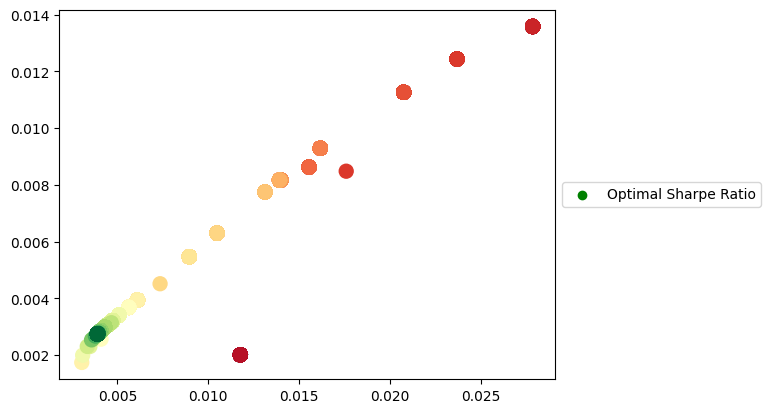
\includegraphics[width=0.5\textwidth]{./images/otimizacao_ibov.png}
                \par \footnotesize Fonte: próprio autor.
            \end{figure}

    \end{frame}
    \note{Convergência}
%-------------------------------------------------------





%-------------------------------------------------------
    \begin{frame}{Otimização com Parâmetros Reais}

        Comparação de modelos:

        \begin{itemize}
            \item Carteira ótima sem restrições reais;
            \item Carteira ótima com restrições reais e início aleatório;
            \item Carteira ótima com restrições reais e heurística.
        \end{itemize}
        
        Cenários: média e desvio padrão dos últimos 15, 30 e 60 dias nos componentes do Ibovespa. 

        Dados: conforme quadro \ref{quadro:coleta_dados} de coleta de dados.

        \begin{quadro}[H]
            \centering
            \caption{Parâmetros de mercado e investimento}
            \label{quadro:parametros}
            \begin{tabular}{ll}
                \hline
                \textbf{Parâmetro} & \textbf{Valor} \\
                \hline
                Capital de Investimento & R\$ 20.000,00 \\
                Valor Monetário Aceitável de Perda Diária & R\$ 100,00 \\
                Quantil da Distribuição Normal Padrão ao Nível de Confiança & 95\% \\
                Quantidade Inicial de Lotes do Ativo & 0 \\
                \hline
            \end{tabular}
            \par \footnotesize Fonte: próprio autor.
        \end{quadro}
        
    \end{frame}
    \note{Parâmetros e dados}
%-------------------------------------------------------





%-------------------------------------------------------
    \begin{frame}{Otimização com Parâmetros Reais}
        
        
        \begin{table}[htbp]
            \centering
            \caption{Resultados da otimização para os três cenários}
            \label{tab:resultados_opt}
            \resizebox{\columnwidth}{!}{%
            \begin{tabular}{clrrrr}
                \hline
                \textbf{Carteira} & \textbf{Método} & \textbf{Retorno} & \textbf{Risco} & \textbf{Sharpe do Otimizador} & \textbf{Tempo (s)} \\ \hline \hline
                15 & Sem Restrições & 15.80 & 16.14 & 0.9791 & 0.42 \\
                15 & Restrições e Aleatório & 3.96 & 39.83 & -0.0849 & 3.81 \\
                15 & Restrições com Heurística & 10.90 & 14.99 & 0.0751 & 3.70 \\
                30 & Sem Restrições & 43.98 & 61.49 & 0.7152 & 0.20 \\
                30 & Restrições e Aleatório & 23.37 & 121.18 & 0.1191 & 3.92 \\
                30 & Restrições com Heurística & 22.80 & 48.41 & 0.2321 & 3.88 \\
                60 & Sem Restrições & 64.01 & 106.91 & 0.5987 & 0.18 \\
                60 & Restrições e Aleatório & 1.15 & 48.36 & -0.1146 & 3.21 \\
                60 & Restrições com Heurística & 15.99 & 66.19 & -0.1700 & 10.13 \\
                \hline
            \end{tabular}%
            }
            \par \footnotesize Fonte: próprio autor.
        \end{table}

    \end{frame}
    \note{Resultados Cenários}
%-------------------------------------------------------





%-------------------------------------------------------
    \begin{frame}{Otimização com Parâmetros Reais}
        
        \begin{figure}[H]
            \centering
            \caption{Densidade de probabilidade das carteiras.}
            \label{fig:densidade_carteiras}
            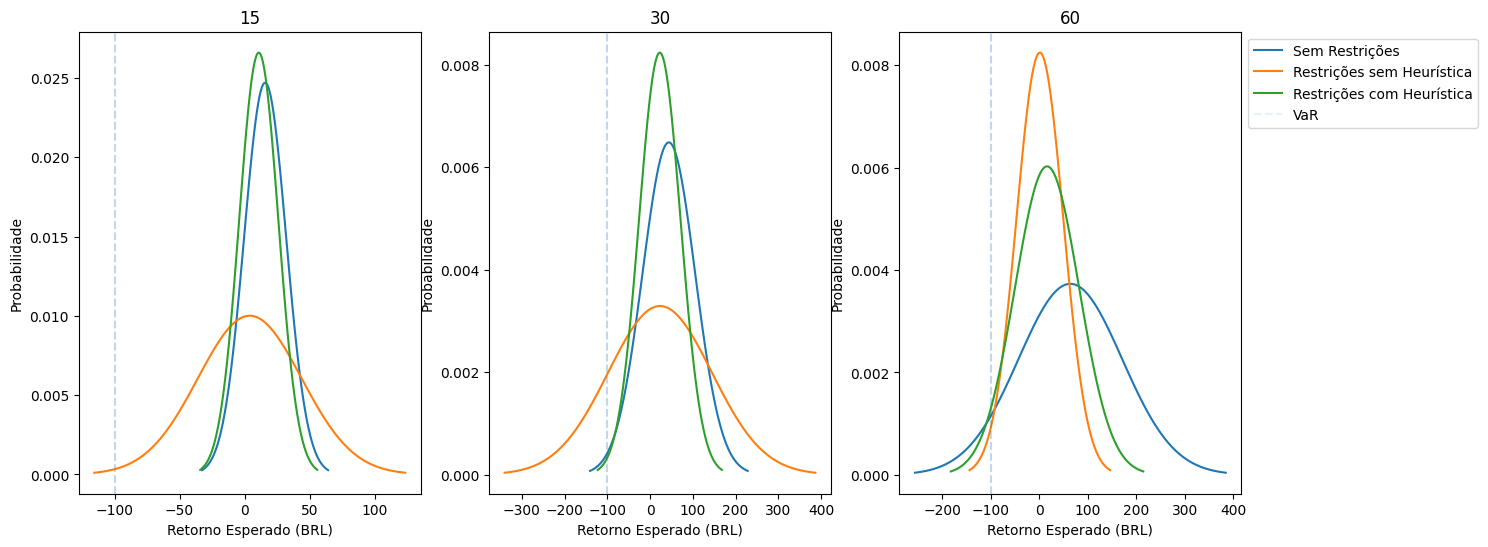
\includegraphics[width=\textwidth]{./images/distribuicao_carteiras.png}
            \par \footnotesize Fonte: próprio autor.
        \end{figure}

    \end{frame}
    \note{Curvas densidade}
%-------------------------------------------------------





%-------------------------------------------------------
    \begin{frame}{Otimização com Parâmetros Reais}
        
        \begin{table}[htbp]
            \centering
            \caption{Alocação da carteira de 30 dias}
            \label{tab:distribuicao_carteira_30}
            \begin{tabular}{rrr}
                \hline
                & Sem Restrições & Restrições com Heurística \\
                \hline\hline
               BRKM5 & 480 & - \\
               ENBR3 & 15620 & 18912 \\
               EQTL3 & 1400 & - \\
               GOLL4 & 80 & - \\
               IRBR3 & 820 & - \\
               JBSS3 & 520 & - \\
               PRIO3 & 540 & - \\
               RAIZ4 & 480 & - \\
               SLCE3 & 40 & - \\
               Livre de Risco & - & 1088 \\
               \hline
            \end{tabular}
            \par \footnotesize Fonte: próprio autor. 
        \end{table}

    \end{frame}
    \note{Alocação de ativos}
%-------------------------------------------------------





%-------------------------------------------------------
    \begin{frame}{Redes Neurais}
        
        \Large

        \begin{columns}
            \begin{column}{0.5\textwidth}

                Após a otimização das carteiras com atualização diária, é realizada a comparação dos retornos gerados pelas carteiras selecionadas no período de análise.

            \end{column}

            \begin{column}{0.5\textwidth}

                \begin{figure}[htbp]
                    \centering
                    \caption{Retornos gerados pelas carteiras.}
                    \label{fig:boxplot_inv}
                    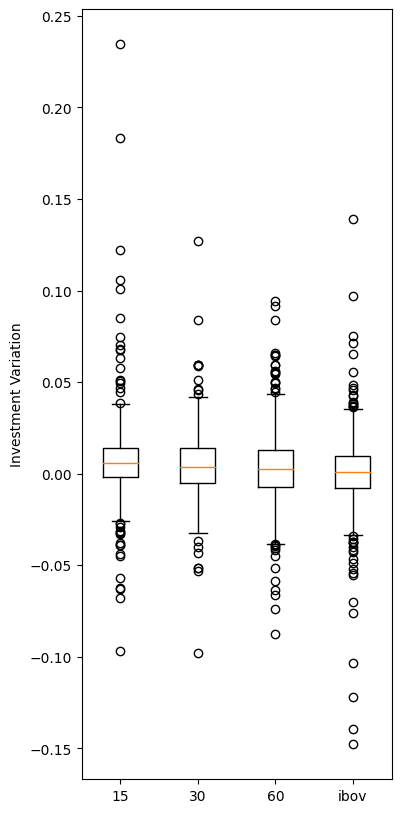
\includegraphics[width=0.4\textwidth]{./images/boxplot_inv.png}
                    \par \footnotesize Fonte: próprio autor.
                \end{figure}

            \end{column}
        \end{columns}

    \end{frame}
    \note{Análise de dados}
%-------------------------------------------------------





%-------------------------------------------------------
    \begin{frame}{Redes Neurais}
        
        \begin{columns}
            \begin{column}{0.5\textwidth}

                \begin{figure}[htbp]
                    \centering
                    \caption{Retorno acumulado das carteiras.}
                    \label{fig:retorno_acumulado}
                    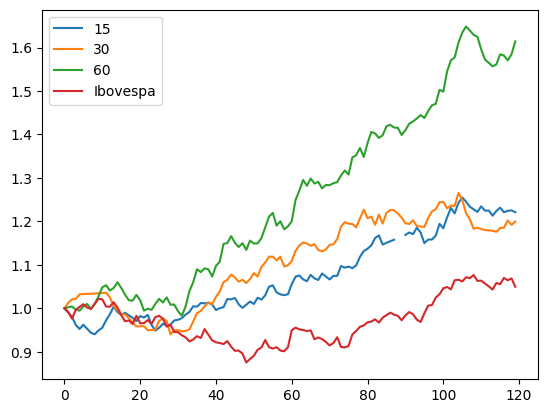
\includegraphics[width=0.9\textwidth]{./images/retorno_acumulado.png}
                    \par \footnotesize Fonte: próprio autor.
                \end{figure}

            \end{column}

            \begin{column}{0.5\textwidth}

                \begin{figure}[htbp]
                    \centering
                    \caption{Porcentagem de sucesso na otimização das carteiras.}
                    \label{fig:success_results}
                    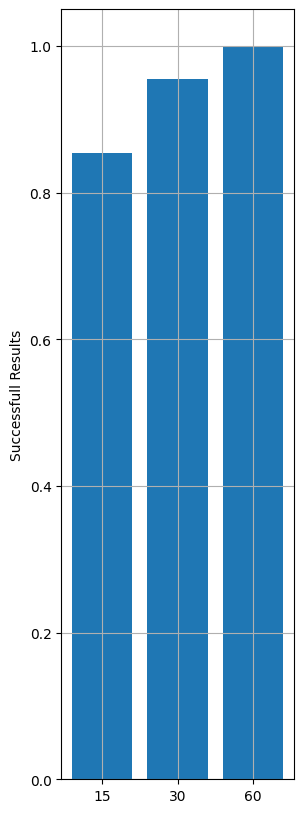
\includegraphics[width=0.3\textwidth]{./images/success_results.png}
                    \par \footnotesize Fonte: próprio autor.
                \end{figure}

            \end{column}
        \end{columns}

    \end{frame}
    \note{Análise de dados}
%-------------------------------------------------------




%-------------------------------------------------------
    \begin{frame}{Redes Neurais}


        \begin{columns}
            \begin{column}{0.5\textwidth}

                Estruturas: 
                \begin{itemize}
                    \item LSTM + Atenção de Bahdanau
                    \item LSTM + Auto Atenção
                    \item GRU + Atenção de Bahdanau
                    \item GRU + Auto Atenção
                \end{itemize}

            \end{column}

            \begin{column}{0.5\textwidth}


                \begin{figure}[htbp]
                    \centering
                    \caption{Acurácia para as redes avaliadas.}
                    \label{fig:accuracy}
                    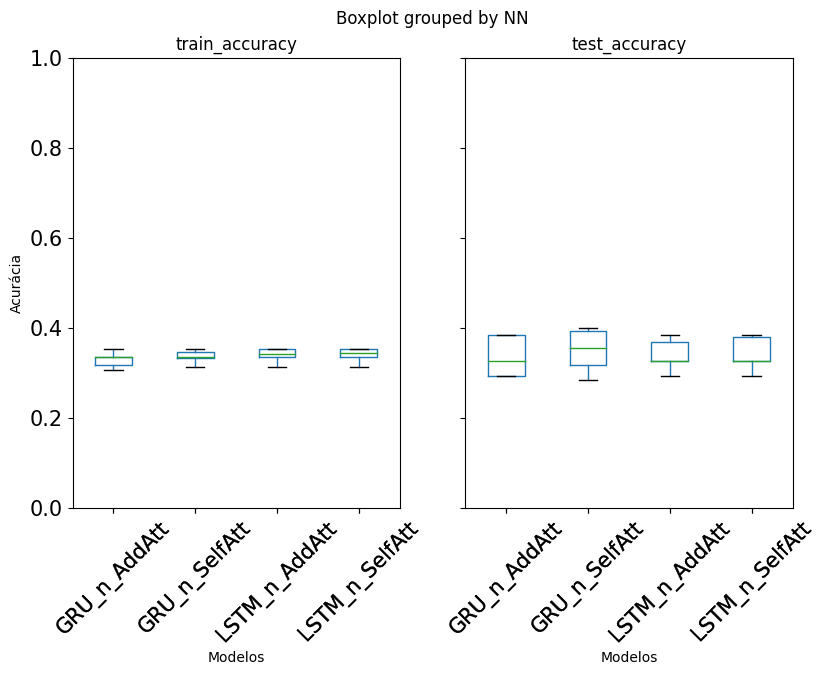
\includegraphics[width=0.98\textwidth]{./images/boxplot_val_01.png}
                    \par \footnotesize Fonte: próprio autor.
                \end{figure}

            \end{column}
        \end{columns}



    \end{frame}
    \note{Acurácia}
%-------------------------------------------------------





%-------------------------------------------------------
    \begin{frame}{Redes Neurais}

        \begin{columns}
            \begin{column}{0.5\textwidth}

                \begin{figure}[htbp]
                    \centering
                    \caption{Frequência dos atributos alvos do teste.}
                    \label{fig:freq}
                    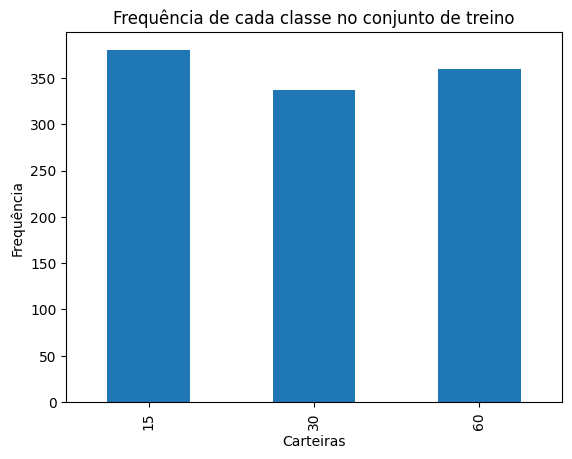
\includegraphics[width=0.98\textwidth]{./images/freq.png}
                    \par \footnotesize Fonte: próprio autor.
                \end{figure}

            \end{column}

            \begin{column}{0.5\textwidth}

                \begin{figure}[htbp]
                    \centering
                    \caption{Acurácia para as redes avaliadas, ampliado.}
                    \label{fig:boxplotval_zoom}
                    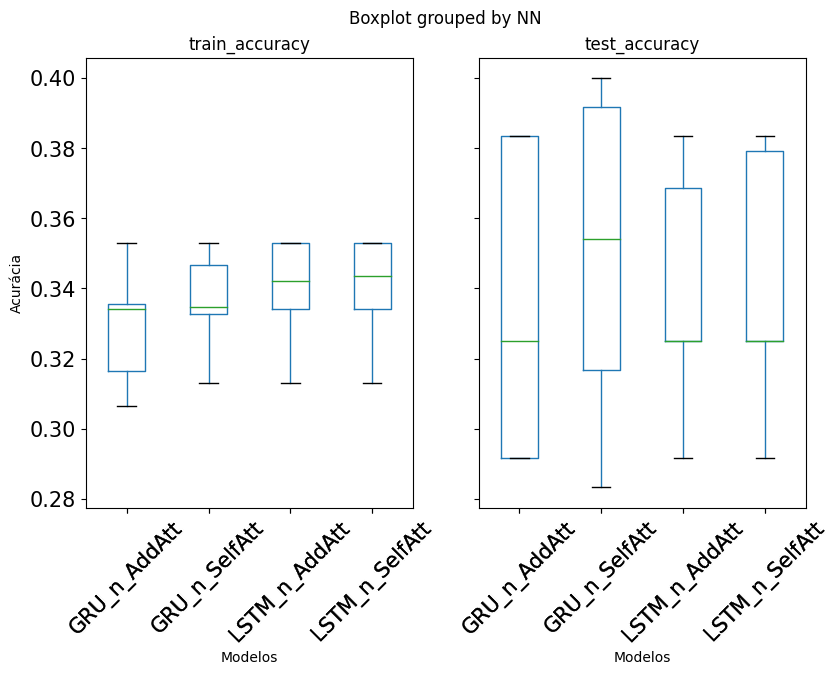
\includegraphics[width=0.98\textwidth]{./images/boxplotval_zoom.png}
                    \par \footnotesize Fonte: próprio autor.
                \end{figure}

            \end{column}
        \end{columns}


    \end{frame}
    \note{Acurácia}
%-------------------------------------------------------





%-------------------------------------------------------
    \begin{frame}{Redes Neurais}

        \begin{figure}[htbp]
            \centering
            \caption{Séries temporais de retorno acumulado geradas pelas predições das redes neurais.}
            \label{fig:backtest_ts}
            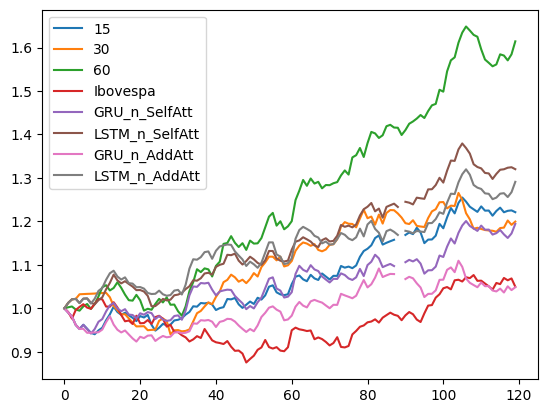
\includegraphics[width=0.5\textwidth]{./images/backtest_ts.png}
            \par \footnotesize Fonte: próprio autor.
        \end{figure}


    \end{frame}
    \note{Séries temporais}
%-------------------------------------------------------





%-------------------------------------------------------
    \begin{frame}{Redes Neurais}

        \begin{table}[htbp]
            \centering
            \caption{Índice Sharpe para as redes avaliadas e as carteiras.}
            \label{tab:sharpe}
            \begin{tabular}{rrrr}
                \hline
                & \textbf{Média} & \textbf{Desvio Padrão} & \textbf{Índice Sharpe} \\ \hline \hline
                GRU\_n\_SelfAtt & 0.0016 & 0.0119 & 0.13 \\
                LSTM\_n\_SelfAtt & 0.0024 & 0.0095 & 0.25 \\
                GRU\_n\_AddAtt & 0.0005 & 0.0105 & 0.04 \\
                LSTM\_n\_AddAtt & 0.0022 & 0.0114 & 0.19 \\
                15 & 0.0017 & 0.0101 & 0.17 \\
                30 & 0.0016 & 0.0108 & 0.15 \\
                60 & 0.0041 & 0.0131 & 0.31 \\
                \hline
                \par \footnotesize Fonte: próprio autor.
            \end{tabular}
        \end{table}

    \end{frame}
    \note{Tabela sharpe}
%-------------------------------------------------------

    %-------------------------------------------------------
\section{Conclusão}
%-------------------------------------------------------


\begin{frame}{Conclusão}

    \Large

    O modelo sem restrições obteve melhor desempenho em tempo de otimização e índice Sharpe, enquanto o modelo com restrições e heurísticas teve desempenho inferior, exceto o modelo com início aleatório.

    As redes neurais não superaram o desempenho das carteiras de investimento, mas superaram o índice Ibovespa. A rede neural LSTM+Atenção de Bahdanau teve o melhor desempenho, embora abaixo da carteira de 60 dias. A rede neural GRU+Atenção de Bahdanau teve o pior desempenho, ficando abaixo do índice Ibovespa em alguns momentos.

\end{frame}
\note{Específicas}


\begin{frame}{Conclusão}

    \Large

    Aplicou-se redes neurais na previsão do índice Sharpe para seleção de carteiras de investimento. Identificado referências relevantes e as técnicas utilizadas. Elaborado modelo de processamento de dados históricos e econômicos. Construídos modelos de otimização e de previsão com redes neurais. Avaliado o desempenho dos modelos.

    Essas descobertas contribuem para o avanço do conhecimento na área de finanças e destacam o potencial das abordagens baseadas em redes neurais na seleção de carteiras de investimento.

    Como sugestões para trabalhos futuros, pode-se a aplicação de dados financeiros de análise técnica no treinamento de redes neurais e também a aplicação de redes neurais em outros modelos de otimização, como o CVaR.


\end{frame}
\note{Gerais e futuros trabalhos}
    
    \miniframesoff

    %================================================
    %----------------BIBLIOGRAFIA
    %================================================
    % \begin{section*}{Referências}

        \begin{frame}[allowframebreaks]{Referências bibliográficas}
        %\nocite{*}

        \setbeamertemplate{bibliography item}[text] 


        \bibliography{referencias/referencias}
        % \printbibliography

        \end{frame}
    % \end{section*}

    %================================================
    %---------------Elementos Pós-textuais
    %================================================

    {\setbeamercolor{palette primary}{fg=DarkBlue, bg=white}
    \begin{frame}[plain,noframenumbering,standout]
        Obrigado! \\
        % Perguntas e Comentários \\
        renandcl@unifei.edu.br
    \end{frame}
    } 

    %================================================
    %----------------FIM DO TEMPLATE
    %================================================


\end{document}